% main.tex
% Dummit & Foote《抽象代数》读书笔记
% 编译：latexmk -xelatex main.tex
\documentclass[10pt]{book}

% ── 加载所有配置 ──
% preamble/packages.tex
\usepackage{ctex}
\usepackage{lipsum}
\usepackage{amsmath, amsthm, amssymb, amsfonts, mathrsfs}
\usepackage{thmtools}
\usepackage{graphicx}
\usepackage{setspace}
\usepackage{geometry}
\usepackage{float}
\usepackage{hyperref}
\usepackage{framed}
\usepackage[dvipsnames]{xcolor}
\usepackage{tikz-cd}
\usepackage[most]{tcolorbox}
\tcbuselibrary{theorems}
\tcbuselibrary{breakable}
\usepackage{enumitem}
\usepackage{fontspec}
\usepackage{xeCJK}

\usepackage{tikz}
\usetikzlibrary{arrows.meta, positioning}

% preamble/colors.tex
% ------------------------------------
% 配色方案：暗红色系主题 + 金饰
% ------------------------------------

% ---- 暗红色系 —— 主结构色 ----
\definecolor{LogicRed}{RGB}{150, 30, 40}
\definecolor{LogicLightRed}{RGB}{210, 120, 130}
\definecolor{LogicDarkRed}{RGB}{80, 15, 20}
\definecolor{LogicAccentRed}{RGB}{185, 50, 60}

\colorlet{RedMain}{LogicRed}        % 主暗红色
\colorlet{RedDark}{LogicDarkRed}    % 深暗红色
\colorlet{RedLight}{LogicLightRed}  % 浅暗红色
\colorlet{RedAccent}{LogicAccentRed}% 强调暗红色

% ---- 暖金色系（Gold）—— 章节扉页装饰 ----
\definecolor{GoldDark}{RGB}{140, 100, 35}
\definecolor{GoldMain}{RGB}{178, 132, 55}
\definecolor{GoldLight}{RGB}{210, 172, 100}
\definecolor{GoldPale}{RGB}{242, 230, 205}

% ---- 兼容旧名称 ----
\colorlet{GreenMain}{LogicRed}
\colorlet{OrangeMain}{LogicRed}

% preamble/theorems.tex
% 基于 thmtools + tcolorbox 的彩色定理环境
% 所有环境共享 theorem 计数器，按 section 编号

\declaretheoremstyle[
spaceabove=6pt, spacebelow=6pt,
headfont=\normalfont\bfseries,
headpunct=,
postheadspace=0.5em,
bodyfont=\normalfont,
headformat=\NAME
]{mycolored}

\declaretheorem[style=mycolored, name=, within=section]{theorem}
\declaretheorem[style=mycolored, name=, sibling=theorem]{lemma}
\declaretheorem[style=mycolored, name=, sibling=theorem]{corollary}
\declaretheorem[style=mycolored, name=, sibling=theorem]{proposition}
\declaretheorem[style=mycolored, name=, sibling=theorem]{definition}
\declaretheorem[style=mycolored, name=, sibling=theorem]{remark}
\declaretheorem[style=mycolored, name=, sibling=theorem]{example}
\declaretheorem[style=mycolored, name=, sibling=theorem]{construction}
\declaretheorem[style=mycolored, name=, sibling=theorem]{problem}
\declaretheorem[style=mycolored, name=, sibling=theorem]{axiom}
\declaretheorem[style=mycolored, name=, sibling=theorem]{note}
\declaretheorem[style=mycolored, name=, sibling=theorem]{ill}
\declaretheorem[style=mycolored, name=, sibling=theorem]{algo}
\declaretheorem[style=mycolored, name=, sibling=theorem]{conjecture}

% ── 修正编号：title 中使用计数器+1 ──
\newcommand{\NextTheoremNum}{\thesection.\number\numexpr\value{theorem}+1\relax}
\newcommand{\NextLemmaNum}{\thesection.\number\numexpr\value{lemma}+1\relax}
\newcommand{\NextCorNum}{\thesection.\number\numexpr\value{corollary}+1\relax}
\newcommand{\NextPropNum}{\thesection.\number\numexpr\value{proposition}+1\relax}
\newcommand{\NextDefNum}{\thesection.\number\numexpr\value{definition}+1\relax}
\newcommand{\NextRemNum}{\thesection.\number\numexpr\value{remark}+1\relax}
\newcommand{\NextExNum}{\thesection.\number\numexpr\value{example}+1\relax}
\newcommand{\NextConNum}{\thesection.\number\numexpr\value{construction}+1\relax}
\newcommand{\NextProblemNum}{\thesection.\number\numexpr\value{problem}+1\relax}
\newcommand{\NextAxiomNum}{\thesection.\number\numexpr\value{axiom}+1\relax}
\newcommand{\NextNoteNum}{\thesection.\number\numexpr\value{note}+1\relax}
\newcommand{\NextIllNum}{\thesection.\number\numexpr\value{ill}+1\relax}
\newcommand{\NextAlgoNum}{\thesection.\number\numexpr\value{algo}+1\relax}
\newcommand{\NextConjNum}{\thesection.\number\numexpr\value{conjecture}+1\relax}

% ════════════════════════════════════════
%  蓝色系：定理、推论、命题、引理
% ════════════════════════════════════════

\AtBeginEnvironment{theorem}{%
	\theoremFont
	\begin{tcolorbox}[enhanced,breakable,
		colback=white,colframe=RedMain,
		arc=4pt,boxrule=0.6pt,leftrule=3pt,
		title=定理 \NextTheoremNum]}
	\AtEndEnvironment{theorem}{\end{tcolorbox}}

\AtBeginEnvironment{corollary}{%
	\theoremFont
	\begin{tcolorbox}[enhanced,breakable,
		colback=white,colframe=RedMain,
		arc=4pt,boxrule=0.6pt,leftrule=3pt,
		title=推论 \NextCorNum]}
	\AtEndEnvironment{corollary}{\end{tcolorbox}}

\AtBeginEnvironment{proposition}{%
	\theoremFont
	\begin{tcolorbox}[enhanced,breakable,
		colback=white,colframe=RedMain,
		arc=4pt,boxrule=0.6pt,leftrule=3pt,
		title=命题 \NextPropNum]}
	\AtEndEnvironment{proposition}{\end{tcolorbox}}

\AtBeginEnvironment{lemma}{%
	\theoremFont
	\begin{tcolorbox}[enhanced,breakable,
		colback=white,colframe=LogicAccentRed,
		arc=4pt,boxrule=0.6pt,leftrule=3pt,
		title=引理 \NextLemmaNum]}
	\AtEndEnvironment{lemma}{\end{tcolorbox}}

\AtBeginEnvironment{conjecture}{%
	\theoremFont
	\begin{tcolorbox}[enhanced,breakable,
		colback=white,colframe=LogicAccentRed,
		arc=4pt,boxrule=0.6pt,leftrule=3pt,
		title=猜想 \NextConjNum]}
	\AtEndEnvironment{conjecture}{\end{tcolorbox}}

% ════════════════════════════════════════
%  深蓝色系：定义、注记、公理
% ════════════════════════════════════════

\AtBeginEnvironment{definition}{%
	\theoremFont
	\begin{tcolorbox}[enhanced,breakable,
		colback=white,colframe=LogicDarkRed,
		arc=4pt,boxrule=0.6pt,leftrule=3pt,
		title=定义 \NextDefNum]}
	\AtEndEnvironment{definition}{\end{tcolorbox}}

\AtBeginEnvironment{remark}{%
	\theoremFont
	\begin{tcolorbox}[enhanced,breakable,
		colback=white,colframe=LogicDarkRed,
		arc=4pt,boxrule=0.6pt,leftrule=3pt,
		title=注记 \NextRemNum]}
	\AtEndEnvironment{remark}{\end{tcolorbox}}

\AtBeginEnvironment{axiom}{%
	\theoremFont
	\begin{tcolorbox}[enhanced,breakable,
		colback=white,colframe=LogicDarkRed,
		arc=4pt,boxrule=0.6pt,leftrule=3pt,
		title=公理 \NextAxiomNum]}
	\AtEndEnvironment{axiom}{\end{tcolorbox}}

% ════════════════════════════════════════
%  无框环境：示例
% ════════════════════════════════════════

\AtBeginEnvironment{example}{%
	\par\theoremFont
	\noindent\textbf{示例 \NextExNum.}\quad
}
\AtEndEnvironment{example}{\par}

% ════════════════════════════════════════
%  蓝框环境：构造、记号、说明、问题、算法
% ════════════════════════════════════════

\AtBeginEnvironment{construction}{%
	\theoremFont
	\begin{tcolorbox}[enhanced,breakable,
		colback=white,colframe=RedMain,
		arc=4pt,boxrule=0.6pt,leftrule=3pt,
		title=构造 \NextConNum]}
	\AtEndEnvironment{construction}{\end{tcolorbox}}

\AtBeginEnvironment{note}{%
	\theoremFont
	\begin{tcolorbox}[enhanced,breakable,
		colback=white,colframe=RedMain,
		arc=4pt,boxrule=0.6pt,leftrule=3pt,
		title=记号 \NextNoteNum]}
	\AtEndEnvironment{note}{\end{tcolorbox}}

\AtBeginEnvironment{problem}{%
	\theoremFont
	\begin{tcolorbox}[enhanced,breakable,
		colback=white,colframe=RedAccent,
		arc=4pt,boxrule=0.6pt,leftrule=3pt,
		title=问题 \NextProblemNum]}
\AtEndEnvironment{problem}{\end{tcolorbox}}

\AtBeginEnvironment{ill}{%
	\theoremFont
	\begin{tcolorbox}[enhanced,breakable,
		colback=white,colframe=RedMain,
		arc=4pt,boxrule=0.6pt,leftrule=3pt,
		title=说明 \NextIllNum]}
	\AtEndEnvironment{ill}{\end{tcolorbox}}

\AtBeginEnvironment{algo}{%
	\theoremFont
	\begin{tcolorbox}[enhanced,breakable,
		colback=white,colframe=LogicAccentRed,
		arc=4pt,boxrule=0.6pt,leftrule=3pt,
		title=算法 \NextAlgoNum]}
	\AtEndEnvironment{algo}{\end{tcolorbox}}

% ════════════════════════════════════════
%  证明环境：楷体，无框，□ 结尾
% ════════════════════════════════════════

\renewenvironment{proof}[1][证明]{%
	\par\proofFont
	\noindent\textbf{#1.}\quad
}{%
	\hfill $\square$\par
}

% ════════════════════════════════════════
%  解答环境：与证明相同样式
% ════════════════════════════════════════

\newenvironment{solution}{%
	\par\proofFont
	\noindent\textbf{解答:}\quad
}{%
	\hfill $\square$\par
}

% ── 行距 ──
\setstretch{1.2}

% preamble/commands.tex
% ── 文本颜色快捷指令 ──
\newcommand{\red}[1]{\textcolor[rgb]{1.00,0.00,0.00}{#1}}
\newcommand{\blue}[1]{\textcolor[rgb]{0.00,0.00,1.00}{#1}}
\newcommand{\green}[1]{\textcolor[rgb]{0.00,1.00,0.00}{#1}}
\newcommand{\darkblue}[1]{\textcolor[rgb]{0.00,0.00,0.50}{#1}}
\newcommand{\darkgreen}[1]{\textcolor[rgb]{0.00,0.37,0.00}{#1}}
\newcommand{\darkred}[1]{\textcolor[rgb]{0.60,0.00,0.00}{#1}}
\newcommand{\brown}[1]{\textcolor[rgb]{0.50,0.30,0.00}{#1}}
\newcommand{\purple}[1]{\textcolor[rgb]{0.50,0.00,0.50}{#1}}

% ── 数域 ──
\newcommand{\R}{\mathbb{R}}
\newcommand{\C}{\mathbb{C}}
\newcommand{\Z}{\mathbb{Z}}
\newcommand{\N}{\mathbb{N}}
\newcommand{\Q}{\mathbb{Q}}
\newcommand{\F}{\mathbb{F}}
\newcommand{\PP}{\mathbb{P}}

% ── 排版辅助 ──
\newcommand{\dd}{\mathrm{d}}
\newcommand{\eps}{\varepsilon}
\newcommand{\abs}[1]{\left| #1 \right|}
\newcommand{\norm}[1]{\left\| #1 \right\|}
\newcommand{\bkt}[1]{\left\langle #1 \right\rangle}
\newcommand{\dif}{\mathop{}\!\mathrm{d}}

% ── 向量 ──
\newcommand{\vect}[1]{\boldsymbol{#1}}
\newcommand{\x}{\boldsymbol{x}}
\newcommand{\y}{\boldsymbol{y}}
\newcommand{\z}{\boldsymbol{z}}

% ── 线性代数 ──
\newcommand{\Ker}{\mathrm{ker}}
\let\Im\relax \DeclareMathOperator{\Im}{Im}
\let\Coker\relax \DeclareMathOperator{\Coker}{Coker}
\let\End\relax \DeclareMathOperator{\End}{End}
\let\Hom\relax \DeclareMathOperator{\Hom}{Hom}
\DeclareMathOperator{\id}{id}
\DeclareMathOperator{\rank}{rank}
\DeclareMathOperator{\Tr}{Tr}
\DeclareMathOperator{\detm}{det}
\DeclareMathOperator{\Span}{span}
\DeclareMathOperator{\lcm}{lcm}

% ── 群论 ──
\DeclareMathOperator{\GL}{GL}
\DeclareMathOperator{\SL}{SL}
\DeclareMathOperator{\SO}{SO}
\DeclareMathOperator{\SU}{SU}
\DeclareMathOperator{\Or}{O}
\DeclareMathOperator{\Sp}{Sp}
\DeclareMathOperator{\Aut}{Aut}
\DeclareMathOperator{\Inn}{Inn}
\DeclareMathOperator{\Out}{Out}
\DeclareMathOperator{\Sym}{Sym}
\DeclareMathOperator{\Alt}{Alt}
\DeclareMathOperator{\Stab}{Stab}
\DeclareMathOperator{\Orbit}{Orbit}
\DeclareMathOperator{\sgn}{sgn}
\DeclareMathOperator{\Fix}{Fix}

% 子群记号
\newcommand{\normal}{\trianglelefteq}
\newcommand{\normalin}{\trianglelefteq}
\newcommand{\ngen}[1]{\langle #1 \rangle}
\newcommand{\gen}[1]{\bkt{#1}}

% 商群
\newcommand{\Zmod}[1]{\mathbb{Z}/#1\mathbb{Z}}

% Sylow 子群
\newcommand{\Syl}{\operatorname{Syl}}
\newcommand{\syl}[2]{\operatorname{Syl}_{#1}(#2)}

% ── 环论 ──
\DeclareMathOperator{\Char}{char}
\DeclareMathOperator{\Nil}{Nil}
\DeclareMathOperator{\Ann}{Ann}
\DeclareMathOperator{\Frac}{Frac}
\DeclareMathOperator{\Spec}{Spec}
\DeclareMathOperator{\mSpec}{MaxSpec}
\newcommand{\ideal}[1]{\langle #1 \rangle}

% ── 域论与 Galois 理论 ──
\DeclareMathOperator{\Gal}{Gal}
\DeclareMathOperator{\Autk}{Aut}
\DeclareMathOperator{\Irr}{Irr}

% ── 模论 ──
\DeclareMathOperator{\Tor}{Tor}
\DeclareMathOperator{\Ext}{Ext}
\DeclareMathOperator{\pd}{pd}
\DeclareMathOperator{\idm}{id}

% ── 直积/直和 ──
\newcommand{\dirprod}{\times}
\newcommand{\dirsum}{\oplus}
\newcommand{\semidirprod}{\rtimes}
% ── 数集（黑板体）──
\newcommand{\RR}{\mathbb{R}}
\newcommand{\NN}{\mathbb{N}}
\newcommand{\ZZ}{\mathbb{Z}}
\newcommand{\QQ}{\mathbb{Q}}
\newcommand{\CC}{\mathbb{C}}
\newcommand{\FF}{\mathbb{F}}
\newcommand{\HH}{\mathbb{H}}
%\newcommand{\PP}{\mathbb{P}}
\newcommand{\EE}{\mathbb{E}}

% ── 花体 ──
\newcommand{\mcA}{\mathcal{A}}
\newcommand{\mcB}{\mathcal{B}}
\newcommand{\mcC}{\mathcal{C}}
\newcommand{\mcD}{\mathcal{D}}
\newcommand{\mcF}{\mathcal{F}}
\newcommand{\mcG}{\mathcal{G}}
\newcommand{\mcI}{\mathcal{I}}
\newcommand{\mcL}{\mathcal{L}}
\newcommand{\mcM}{\mathcal{M}}
\newcommand{\mcN}{\mathcal{N}}
\newcommand{\mcO}{\mathcal{O}}
\newcommand{\mcP}{\mathcal{P}}
\newcommand{\mcS}{\mathcal{S}}
\newcommand{\mcT}{\mathcal{T}}
\newcommand{\mcU}{\mathcal{U}}

% ── 哥特体 ──
\newcommand{\mfa}{\mathfrak{a}}
\newcommand{\mfb}{\mathfrak{b}}
\newcommand{\mfg}{\mathfrak{g}}
\newcommand{\mfh}{\mathfrak{h}}
\newcommand{\mfm}{\mathfrak{m}}
\newcommand{\mfn}{\mathfrak{n}}
\newcommand{\mfp}{\mathfrak{p}}
\newcommand{\mfq}{\mathfrak{q}}
\newcommand{\mfr}{\mathfrak{r}}
\newcommand{\mfs}{\mathfrak{s}}

% ── 群论 ──
%\DeclareMathOperator{\Aut}{Aut}
\DeclareMathOperator{\Hol}{Hol}
%\DeclareMathOperator{\Inn}{Inn}
%\DeclareMathOperator{\End}{End}
%\DeclareMathOperator{\Hom}{Hom}
%\DeclareMathOperator{\Syl}{Syl}
%\DeclareMathOperator{\Stab}{Stab}
%\DeclareMathOperator{\sgn}{sgn}
%\DeclareMathOperator{\GL}{GL}
%\DeclareMathOperator{\SL}{SL}
\DeclareMathOperator{\PSL}{PSL}
%\DeclareMathOperator{\SO}{SO}
\DeclareMathOperator{\charac}{char}

% ── 环论与模论 ──
%\DeclareMathOperator{\Spec}{Spec}
\DeclareMathOperator{\nilrad}{nil}
\DeclareMathOperator{\rad}{rad}
\DeclareMathOperator{\Jac}{Jac}
%\DeclareMathOperator{\Ann}{Ann}
%\DeclareMathOperator{\Frac}{Frac}
\DeclareMathOperator{\coker}{coker}
%\DeclareMathOperator{\Ext}{Ext}
%\DeclareMathOperator{\Tor}{Tor}

% ── 域论 ──
%\DeclareMathOperator{\Gal}{Gal}
%\DeclareMathOperator{\Tr}{Tr}
\DeclareMathOperator{\Nm}{Nm}

% ── 常用 ──
%\DeclareMathOperator{\id}{id}
\DeclareMathOperator{\im}{im}
\newcommand{\divides}{\mid}
\newcommand{\ndivides}{\nmid}
%\newcommand{\normal}{\trianglelefteq}
\newcommand{\semidirect}{\rtimes}
\newcommand{\dsum}{\bigoplus}
\newcommand{\tensor}{\otimes}
% preamble/geometry.tex
\geometry{
	textheight=9in,
	textwidth=5.5in,
	top=1in,
	headheight=12pt,
	headsep=25pt,
	footskip=30pt
}
% -------------------------------
% 全局正文字体（英文 + 中文）
% -------------------------------
\setmainfont{Times New Roman}    % 英文正文
\setCJKmainfont{SimSun}          % 中文正文：宋体

% -------------------------------
% 定理环境中文字体：仿宋
% -------------------------------
\setCJKfamilyfont{theoremCJK}{FangSong}
\newcommand{\theoremFont}{\CJKfamily{theoremCJK}}

% -------------------------------
% 证明环境中文字体：楷体
% -------------------------------
\setCJKfamilyfont{proofCJK}{KaiTi}
\newcommand{\proofFont}{\CJKfamily{proofCJK}}

\setCJKmainfont{SimSun}[AutoFakeBold={3}]
\setCJKfamilyfont{theoremCJK}{FangSong}[AutoFakeBold={2.5}]
\setCJKfamilyfont{proofCJK}{KaiTi}[AutoFakeBold={2.5}]

% preamble/chapter.title.tex
% 章节扉页设计（蓝色系）：全纸面图片 + 彩条 + 介绍区

\RequirePackage{tikz}
\RequirePackage{graphicx}
\RequirePackage{etoolbox}
\RequirePackage{setspace}

\makeatletter

% -------- 每章图片接口 --------
\newcommand{\chapterimage}{}
\newcommand{\setchapterimage}[1]{\gdef\chapterimage{#1}}

% -------- 章节介绍接口 --------
\newcommand{\chapterintro}{}
\newcommand{\setchapterintro}[1]{\gdef\chapterintro{#1}}

% -------- 版式参数 --------
\newlength{\ChapterTopImageHeight}
\setlength{\ChapterTopImageHeight}{14.2cm}

\newlength{\ChapterRibbonHeight}
\setlength{\ChapterRibbonHeight}{2.35cm}

\newlength{\ChapterIntroTopSep}
\setlength{\ChapterIntroTopSep}{1.15cm}

\newlength{\ChapterIntroWidth}
\setlength{\ChapterIntroWidth}{\dimexpr\textwidth+0.6cm\relax}

\newlength{\ChapterIntroLeft}
\setlength{\ChapterIntroLeft}{\dimexpr\paperwidth/2-\ChapterIntroWidth/2\relax}

\newlength{\ChapterImageMid}
\setlength{\ChapterImageMid}{\dimexpr\ChapterTopImageHeight/2\relax}

\newlength{\ChapterImageShadeTop}
\setlength{\ChapterImageShadeTop}{\dimexpr\ChapterTopImageHeight-1.0cm\relax}

\newlength{\ChapterRibbonMid}
\setlength{\ChapterRibbonMid}{\dimexpr\ChapterTopImageHeight+\ChapterRibbonHeight/2\relax}

\newlength{\ChapterRibbonBottom}
\setlength{\ChapterRibbonBottom}{\dimexpr\ChapterTopImageHeight+\ChapterRibbonHeight\relax}

\newlength{\ChapterIntroTop}
\setlength{\ChapterIntroTop}{\dimexpr\ChapterTopImageHeight+\ChapterRibbonHeight+\ChapterIntroTopSep\relax}

% 章节介绍排版
\newcommand{\ChapterIntroBlock}{%
	\ifdefempty{\chapterintro}{%
		\vspace*{6.4cm}%
	}{%
		{\Large\bfseries\color{RedMain} 本章导读\par}%
		\vspace{0.55cm}%
		{\setstretch{1.35}\large\itshape\color{RedDark}\chapterintro\par}%
	}%
}

% 通用章节扉页：#1 = 彩条中的标题文字
\newcommand{\ChapterTitlePage}[1]{%
	\thispagestyle{empty}%
	\vspace*{-\baselineskip}%
	\begin{tikzpicture}[remember picture,overlay]
		% ====== 上部：整页宽图片区 ======
		\ifdefempty{\chapterimage}{%
			\shade[top color=RedMain!18,bottom color=RedMain!6]
				(current page.north west) rectangle
				([yshift=-\ChapterTopImageHeight]current page.north east);
		}{%
			\node[anchor=north west,inner sep=0pt,outer sep=0pt]
				at (current page.north west)
				{\includegraphics[
					width=\paperwidth,
					height=\ChapterTopImageHeight
				]{\chapterimage}};
		}%
		% 图片底部渐变
		\shade[top color=black!0,bottom color=black!22]
			([yshift=-\ChapterImageShadeTop]current page.north west) rectangle
			([yshift=-\ChapterTopImageHeight]current page.north east);
		
		% ====== 中部：全宽蓝色彩条 ======
		\fill[RedMain!94]
			([yshift=-\ChapterTopImageHeight]current page.north west) rectangle
			([yshift=-\ChapterRibbonBottom]current page.north east);
		\fill[GoldMain!75]
			([yshift=-\ChapterTopImageHeight]current page.north west) rectangle
			([xshift=0.18cm,yshift=-\ChapterRibbonBottom]current page.north west);
		\fill[GoldMain!75]
			([xshift=-0.18cm,yshift=-\ChapterTopImageHeight]current page.north east) rectangle
			([yshift=-\ChapterRibbonBottom]current page.north east);
		\node[text=white,font=\bfseries\huge,align=center,text width=\dimexpr\paperwidth-2.2cm\relax]
			at ([yshift=-\ChapterRibbonMid]current page.north)
			{#1};
		\draw[GoldMain!45,line width=0.7pt]
			([yshift=-\ChapterRibbonBottom]current page.north west) --
			([yshift=-\ChapterRibbonBottom]current page.north east);
		
		% ====== 下部：章节介绍区域 ======
		\coordinate (introNW) at
			([xshift=\ChapterIntroLeft,
			  yshift=-\ChapterIntroTop]
			 current page.north west);
		\draw[GoldMain!45,line width=0.8pt] (introNW) -- ++(\ChapterIntroWidth,0);
		\node[anchor=north west,inner sep=0pt,outer sep=0pt,text width=\ChapterIntroWidth,align=left]
			at ([yshift=-0.55cm]introNW)
			{\ChapterIntroBlock};
	\end{tikzpicture}%
	\vspace*{\fill}%
	\clearpage%
}

% numbered chapter 标题
\def\@makechapterhead#1{%
	\if@mainmatter
		\ChapterTitlePage{第\thechapter 章\quad #1}%
	\else
		\vspace*{50pt}%
		{\noindent\huge\bfseries #1\par}%
		\vskip 40pt%
	\fi
}

% unnumbered chapter 标题
\def\@makeschapterhead#1{%
	\if@mainmatter
		\ChapterTitlePage{#1}%
	\else
		\vspace*{50pt}%
		{\noindent\huge\bfseries #1\par}%
		\vskip 40pt%
	\fi
}

\makeatother

% preamble/part.title.tex
% Part 扉页设计（蓝金配色）

\RequirePackage{tikz}
\RequirePackage{graphicx}
\RequirePackage{etoolbox}
\RequirePackage{setspace}

\makeatletter

% -------- 每 Part 图片接口 --------
\gdef\partimage{}
\newcommand{\setpartimage}[1]{\gdef\partimage{#1}}

% -------- Part 简介接口 --------
\gdef\partintro{}
\newcommand{\setpartintro}[1]{\gdef\partintro{#1}}

% -------- 版式参数 --------
\newlength{\PartRibbonHeight}
\setlength{\PartRibbonHeight}{2.35cm}

\newlength{\PartContentTop}
\setlength{\PartContentTop}{\dimexpr\PartRibbonHeight+1.2cm\relax}

\newlength{\PartDividerY}
\setlength{\PartDividerY}{\dimexpr\PartRibbonHeight+6.8cm\relax}

% -------- 左上 Part 标题 block --------
\newcommand{\PartTitleBlock}[2]{%
	\ifdefempty{#1}{%
		\fill[GoldMain!55]
		([xshift=1.8cm,yshift=-\PartContentTop]current page.north west)
		-- ++(0.22,0.22) -- ++(-0.22,0.22) -- ++(-0.22,-0.22) -- cycle;
	}{%
		\node[anchor=north west,text=GoldMain!72,font=\fontsize{52}{62}\bfseries]
		at ([xshift=1.8cm,yshift=-\PartContentTop]current page.north west)
		{#1};
		\node[anchor=north west,text=GoldMain!48,font=\Large\bfseries]
		at ([xshift=1.8cm,yshift=-\PartContentTop-3.1cm]current page.north west)
		{Part};
	}%
	\node[anchor=north west,text=RedDark,font=\fontsize{22}{28}\bfseries,
	text width=8cm,align=left]
	at ([xshift=1.8cm,yshift=-\PartContentTop-4.4cm]current page.north west)
	{#2};
}

% -------- 右上简介 block --------
\newcommand{\PartIntroBlock}{%
	\ifdefempty{\partintro}{}{%
		\node[anchor=north east,text=RedMain!80,font=\Large\bfseries]
		at ([xshift=-1.8cm,yshift=-\PartContentTop]current page.north east)
		{简\quad 介};
		\node[anchor=north east,text=RedDark!55,font=\large\itshape,
		text width=7.4cm,align=right,inner sep=0pt]
		at ([xshift=-1.8cm,yshift=-\PartContentTop-1.5cm]current page.north east)
		{\setstretch{1.45}\partintro};
	}%
}

% -------- Part 扉页 --------
\newcommand{\PartTitlePage}[2]{%
	\thispagestyle{empty}%
	\vspace*{-\baselineskip}%
	\begin{tikzpicture}[remember picture,overlay]
		% 顶部全宽深蓝横条
		\fill[RedMain!94]
		(current page.north west) rectangle
		([yshift=-\PartRibbonHeight]current page.north east);
		\fill[GoldMain!75]
		(current page.north west) rectangle
		([xshift=0.18cm,yshift=-\PartRibbonHeight]current page.north west);
		\fill[GoldMain!75]
		([xshift=-0.18cm]current page.north east) rectangle
		([yshift=-\PartRibbonHeight]current page.north east);
		
		% 左上：Part 编号 + 标题
		\PartTitleBlock{#1}{#2}
		
		% 右上：简介区域
		\PartIntroBlock
		
		% 金色装饰虚线
		\draw[GoldMain!20,line width=0.5pt,dash pattern=on 3pt off 5pt]
		([xshift=11.0cm,yshift=-\PartContentTop]current page.north west) --
		([xshift=11.0cm,yshift=-\PartDividerY+0.3cm]current page.north west);
		
		% 金色分割线
		\draw[GoldMain!42,line width=0.7pt]
		([yshift=-\PartDividerY]current page.north west) --
		([yshift=-\PartDividerY]current page.north east);
		\fill[GoldMain!50]
		([yshift=-\PartDividerY]current page.north west) circle (1.8pt);
		\fill[GoldMain!50]
		([yshift=-\PartDividerY]current page.north east) circle (1.8pt);
		\fill[GoldMain!60]
		([yshift=-\PartDividerY]current page.north)
		-- ++(0.13,0.13) -- ++(-0.13,0.13) -- ++(-0.13,-0.13) -- cycle;
		
		% 下方全宽图片
		\ifdefempty{\partimage}{%
			\shade[top color=RedMain!12,bottom color=RedMain!3]
			([yshift=-\PartDividerY]current page.north west) rectangle
			(current page.south east);
		}{%
			\node[anchor=north west,inner sep=0pt,outer sep=0pt]
			at ([yshift=-\PartDividerY]current page.north west)
			{\includegraphics[
				width=\paperwidth,
				height=\dimexpr\paperheight-\PartDividerY\relax
				]{\partimage}};
		}%
	\end{tikzpicture}%
	\clearpage%
	\if@twoside
	\if@openright
	\null
	\thispagestyle{empty}%
	\newpage
	\fi
	\fi
}

% 重定义 \@part
\def\@part[#1]#2{%
	\ifnum \c@secnumdepth >-2\relax
	\refstepcounter{part}%
	\addcontentsline{toc}{part}{\thepart\hspace{1em}#1}%
	\else
	\addcontentsline{toc}{part}{#1}%
	\fi
	\markboth{}{}%
	\PartTitlePage{\thepart}{#2}%
	\@endpart
}

% 重定义 \@spart（无编号 Part）
\def\@spart#1{%
	\PartTitlePage{}{#1}%
	\@endpart
}

\def\@endpart{%
	\if@tempswa
	\twocolumn
	\fi
}

\makeatother

% preamble/cover.tex
% 简化版封面 —— Dummit 抽象代数读书笔记
% 蓝金配色，保留九层 TikZ 设计骨架

\makeatletter
\providecommand{\@coverimage}{}
\newcommand{\coverimage}[1]{\renewcommand{\@coverimage}{#1}}

\newcommand{\makecover}{%
\begin{titlepage}
\thispagestyle{empty}

% ============================================================
%  第一层：左侧深蓝色竖条 + 装饰
% ============================================================

\begin{tikzpicture}[remember picture,overlay]
  \fill[RedDark!95]
    (current page.south west) rectangle
    ([xshift=2.8cm]current page.north west);
  \shade[top color=RedDark!90, bottom color=RedDark!95]
    ([xshift=0cm,yshift=-4cm]current page.north west) rectangle
    ([xshift=2.8cm]current page.north west);
  \shade[bottom color=RedDark!90, top color=RedDark!95]
    ([xshift=0cm,yshift=4cm]current page.south west) rectangle
    ([xshift=2.8cm]current page.south west);
  \draw[RedAccent!50,line width=1pt]
    ([xshift=2.8cm]current page.south west) --
    ([xshift=2.8cm]current page.north west);
  \draw[RedLight!25,line width=0.4pt]
    ([xshift=0.4cm]current page.south west) --
    ([xshift=0.4cm]current page.north west);
  \foreach \y/\r/\o in {
    0.08/1.1/0.07, 0.22/0.7/0.11, 0.40/1.4/0.06,
    0.55/0.55/0.10, 0.68/0.9/0.08, 0.82/0.6/0.11, 0.93/0.75/0.09
  } {
    \fill[white, opacity=\o]
      ([xshift=1.4cm, yshift=-\y\paperheight]current page.north west)
      circle (\r cm);
  }
  \draw[white, line width=0.3pt, opacity=0.18]
    ([xshift=0.5cm]current page.north west) --
    ([xshift=0.5cm]current page.south west);
  \draw[white, line width=0.3pt, opacity=0.18]
    ([xshift=2.1cm]current page.north west) --
    ([xshift=2.1cm]current page.south west);
\end{tikzpicture}

% ============================================================
%  第二层：顶部/底部装饰金线
% ============================================================
\begin{tikzpicture}[remember picture,overlay]
  \draw[GoldMain!50,line width=0.6pt]
    ([xshift=3.0cm,yshift=-1.6cm]current page.north west) --
    ([xshift=-2.0cm,yshift=-1.6cm]current page.north east);
  \foreach \x in {3.5,7,10.5,14} {
    \fill[GoldMain!60]
      ([xshift=\x cm,yshift=-1.45cm]current page.north west)
      circle (1.5pt);
  }
  \draw[GoldMain!40,line width=0.5pt]
    ([xshift=3.0cm,yshift=2.2cm]current page.south west) --
    ([xshift=-1.5cm,yshift=2.2cm]current page.south east);
  \foreach \x in {4,8,12} {
    \fill[GoldMain!45]
      ([xshift=\x cm,yshift=2.35cm]current page.south west)
      circle (1.2pt);
  }
\end{tikzpicture}

% ============================================================
%  第三层：右上角装饰几何图形
% ============================================================
\begin{tikzpicture}[remember picture,overlay]
  \draw[GoldMain!30,line width=0.7pt]
    ([xshift=-2.5cm,yshift=-2.5cm]current page.north east)
    circle (22pt);
  \draw[RedAccent!30,line width=0.5pt]
    ([xshift=-2.5cm,yshift=-2.5cm]current page.north east)
    circle (14pt);
  \fill[GoldMain!50]
    ([xshift=-2.5cm,yshift=-2.5cm]current page.north east)
    circle (2.5pt);
  \foreach \ang in {0,90,180,270} {
    \draw[GoldMain!25,line width=0.4pt]
      ([xshift=-2.5cm,yshift=-2.5cm]current page.north east)
      -- ++(\ang:28pt);
  }
  \foreach \ang in {45,135,225,315} {
    \draw[RedAccent!20,line width=0.3pt]
      ([xshift=-2.5cm,yshift=-2.5cm]current page.north east)
      -- ++(\ang:26pt);
  }
\end{tikzpicture}

% ============================================================
%  第四层：左下角装饰曲线
% ============================================================
\begin{tikzpicture}[remember picture,overlay]
  \draw[GoldMain!15,line width=0.5pt,smooth]
    ([xshift=3.5cm,yshift=3.0cm]current page.south west)
    to[out=30,in=210] ++(3.0,2.0);
  \draw[RedAccent!15,line width=0.5pt,smooth]
    ([xshift=3.3cm,yshift=3.0cm]current page.south west)
    to[out=35,in=205] ++(3.2,2.2);
  \draw[RedMain!12,line width=0.5pt,smooth]
    ([xshift=3.5cm,yshift=4.0cm]current page.south west)
    to[out=-15,in=195] ++(2.5,-1.5);
\end{tikzpicture}

% ============================================================
%  第五层：公式背景区
% ============================================================
\begin{tikzpicture}[remember picture,overlay]
  \shade[top color=GoldPale!40, bottom color=GoldPale!25]
    ([xshift=3.3cm,yshift=-3cm]current page.north west) rectangle
    ([xshift=-1.5cm,yshift=2.5cm]current page.south east);
  \draw[GoldMain!30,line width=0.4pt]
    ([xshift=3.3cm,yshift=-3cm]current page.north west) rectangle
    ([xshift=-1.5cm,yshift=2.5cm]current page.south east);
  
  % 代数学经典公式
  \node[anchor=west,RedMain!70] at ([xshift=3.7cm,yshift=-3.5cm]current page.north west)
    {$\displaystyle G/\Ker\phi\;\cong\;\Im\phi$};
  \node[anchor=west,RedAccent!65] at ([xshift=3.8cm,yshift=-4.8cm]current page.north west)
    {$\displaystyle |G|=|H|\cdot[G:H]$};
  \node[anchor=west,GoldMain!75] at ([xshift=3.9cm,yshift=-6.1cm]current page.north west)
    {$\displaystyle \Aut(\Z/n\Z)\cong(\Z/n\Z)^{\times}$};
  \node[anchor=west,RedMain!55] at ([xshift=4.0cm,yshift=-7.4cm]current page.north west)
    {$\displaystyle \Gal(E/F)\cong G$};
  \node[anchor=west,RedAccent!50] at ([xshift=3.7cm,yshift=-8.7cm]current page.north west)
    {$\displaystyle R/I\ \text{域}\ \Longleftrightarrow\ I\ \text{极大理想}$};
  
  \foreach \y/\c in {-3.5/RedMain!35, -4.8/RedAccent!30, -6.1/GoldMain!35, -7.4/RedMain!30, -8.7/RedAccent!25} {
    \fill[\c]
      ([xshift=-2.0cm,yshift=\y cm]current page.north west)
      circle (1.8pt);
  }
\end{tikzpicture}

% ============================================================
%  第六层：标题区
% ============================================================
\vspace*{2cm}

\hspace*{3.3cm}
\begin{minipage}{0.7\textwidth}
  {\large\bfseries\color{RedAccent} Dummit \& Foote 抽象代数\quad 读书笔记\par}
  
  \vspace{0.3cm}
  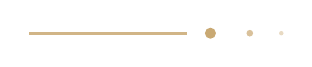
\begin{tikzpicture}
    \draw[GoldMain!60,line width=1.2pt] (0,0) -- (2.0,0);
    \fill[GoldMain!70] (2.3,0) circle (2pt);
    \fill[GoldMain!50] (2.8,0) circle (1.2pt);
    \fill[GoldMain!30] (3.2,0) circle (0.8pt);
  \end{tikzpicture}
  
  \vspace{0.8cm}
  {\Huge\bfseries\color{RedDark} \@title\par}
  
  \vspace{0.6cm}
  {\Large\color{RedMain!70} \@author\par}
  
  \vspace{0.4cm}
  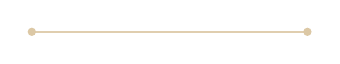
\begin{tikzpicture}
    \draw[GoldMain!40,line width=0.7pt] (0,0) -- (3.5,0);
    \fill[GoldMain!45] (0,0) circle (1.5pt);
    \fill[GoldMain!45] (3.5,0) circle (1.5pt);
  \end{tikzpicture}
  
  \vspace{0.8cm}
  {\large\color{GoldMain!85} 译注：万一之\par}
  \vspace{0.5cm}
  {\normalsize\color{RedDark!60} 原书：\textit{Abstract Algebra}, 3rd ed.\par}

\end{minipage}

% ============================================================
%  第七层：底部图片
% ============================================================
\ifdefempty{\@coverimage}{}{
	\begin{tikzpicture}[remember picture,overlay]
		\node[anchor=south west,inner sep=0pt,outer sep=0pt]
		at ([xshift=3.3cm,yshift=3.05cm]current page.south west)
		{
			\includegraphics[
			width=\dimexpr\paperwidth-4.8cm\relax
			]{\@coverimage}
		};
	\end{tikzpicture}
}

% ============================================================
%  第八层：散落装饰点
% ============================================================
\begin{tikzpicture}[remember picture,overlay]
  \fill[GoldMain!20] ([xshift=-3.0cm,yshift=-9.5cm]current page.north west) circle (1.0pt);
  \fill[RedAccent!20] ([xshift=-3.8cm,yshift=-9.8cm]current page.north west) circle (0.7pt);
  \fill[RedMain!15] ([xshift=-4.0cm,yshift=3.5cm]current page.south west) circle (1.2pt);
  \fill[GoldMain!15] ([xshift=-5.5cm,yshift=4.0cm]current page.south west) circle (0.9pt);
\end{tikzpicture}

\end{titlepage}
}
\makeatother


% ── 文档元信息与封面 ──
\title{抽象代数笔记}
\author{Abstract Algebra Notes}
\date{\today}
\coverimage{figure/封面.png}

\begin{document}

\makecover

\frontmatter
	\tableofcontents
	\newpage
	
\mainmatter
\setcounter{page}{1}

% ═══════════════════════════════════════════════════════
%  Part I：群论 (Group Theory)
% ═══════════════════════════════════════════════════════
\setpartimage{}
\setpartintro{从群的基本定义出发，系统学习子群、商群、群同态、群作用以及 Sylow 定理等群论核心内容，建立抽象代数的第一块基石。}
\part{群论}

%% !TEX root = ../main.tex
\setchapterimage{}
\setchapterintro{本章从二元运算与群公理出发,引入子群、循环群、对称群、二面体群等基本例子,建立群的初等性质,并介绍同态与群作用的基本概念.对应原书 Chapter 1: Introduction to Groups.}
\chapter{群论导引}
\section{基本公理与例子}
\begin{definition}
	\begin{enumerate}
		\item 集合 $G$ 上的一个\textbf{二元运算} $*$ 是一个函数 $*:G\times G\to G$.对任意 $a,b\in G$,我们把 $*(a,b)$ 写作 $a*b$.
		\item 若集合 $G$ 上的二元运算 $*$ 满足对所有 $a,b,c\in G$,都有
		\[
		a*(b*c)=(a*b)*c,
		\]
		则称 $*$ 是\textbf{结合的}.
		\item 若 $*$ 是集合 $G$ 上的二元运算,若 $G$ 中元素 $a,b$ 满足 $a*b=b*a$,则称 $a$ 与 $b$ \textbf{交换}.若对所有 $a,b\in G$ 都有 $a*b=b*a$,则称 $*$（或称 $G$）是\textbf{交换的}.
	\end{enumerate}
\end{definition}
\begin{example}
	$+,\times$ 是$\Z,\Q,\R,\C$上的交换且结合二元运算,但是$-$是$\Z,\Q,\R,\C$上的非交换二元运算,进一步的$-$不是$\Z_+$上的二元运算
\end{example}
设 $*$ 是集合 $G$ 上的二元运算,且 $H$ 是 $G$ 的子集.若 $*$ 到 $H$ 的限制是 $H$ 上的二元运算,即对所有 $a,b\in H$ 都有 $a*b\in H$,则称 $H$ 对 $*$ \textbf{封闭}.注意,如果 $*$ 是 $G$ 上的结合（相应地,交换）二元运算,并且 $*$ 限制到 $G$ 的某个子集 $H$ 上是 $H$ 的二元运算,那么 $*$ 在 $H$ 上也自动是结合的（相应地,交换的）


\begin{definition}
	\begin{enumerate}[label=(\arabic*)]
	\item \textbf{群}是一个有序对 $(G,*)$,其中 $G$ 是一个集合,$*$ 是 $G$ 上的二元运算,并满足以下公理：
	\begin{enumerate}[label=(\roman*)]
		\item 对所有 $a,b,c\in G$,$(a*b)*c=a*(b*c)$,即 $*$ 是结合的；
		\item 存在 $G$ 中的元素 $e$,称为 $G$ 的\textbf{单位元},使得对所有 $a\in G$,都有 $a*e=e*a=a$；
		\item 对每个 $a\in G$,存在 $G$ 中的元素 $a^{-1}$,称为 $a$ 的\textbf{逆元},使得 $a*a^{-1}=a^{-1}*a=e$.
	\end{enumerate}
	\item 若群 $(G,*)$ 满足对所有 $a,b\in G$ 都有 $a*b=b*a$,则称它是\textbf{阿贝尔的}（或\textbf{交换的}）.
\end{enumerate}

\end{definition}
在明确了运算$*$的情况下,直接简称$G$是一个群.若$G$是一个有限集,就称$G$是有限群.由公理$(ii)$保证群是非空的.

\begin{example}
	\begin{enumerate}[label=(\arabic*)]
		\item $\Z$、$\Q$、$\R$ 和 $\C$ 在 $+$ 下是群,其中 $e=0$,并且对所有 $a$,$a^{-1}=-a$.
		\item $\Q-\{0\}$、$\R-\{0\}$、$\C-\{0\}$、$\Q^+$、$\R^+$ 在 $\times$ 下是群,其中 $e=1$,并且对所有 $a$,$a^{-1}=1/a$.但是要注意,$\Z-\{0\}$ 在 $\times$ 下不是群,因为虽然 $\times$ 是 $\Z-\{0\}$ 上的结合二元运算,但元素 $2$（例如）在 $\Z-\{0\}$ 中没有逆元.
	\end{enumerate}
\end{example}
下面我们再定义一个常用的结构,用于举例子,我们假设读者已经具备了初步的数论知识,知道整除,同余的定义.

\begin{definition}
	对一个已经固定下来的正整数$n$,定义$\overline{a}$；这称为 $a$ 模 $n$ 的\textbf{同余类}或\textbf{剩余类},它由与 $a$ 相差 $n$ 的整数倍的所有整数组成,即
	\[
	\overline{a}=\{a+kn\mid k\in\Z\}
	=\{a,\ a\pm n,\ a\pm2n,\ a\pm3n,\ldots\}.
	\]
	
	模 $n$ 恰有 $n$ 个不同的等价类,即
	\[
	\overline{0},\overline{1},\overline{2},\ldots,\overline{n-1},
	\]
	它们由除以 $n$ 后可能出现的余数决定,并且这些剩余类划分整数集 $\Z$.在这个等价关系下的等价类集合记为 $\Z/n\Z$,称为\textbf{模 $n$ 的整数}（或\textbf{模 $n$ 整数}）.

\end{definition}
我们可以为 $\Z/n\Z$ 的元素定义加法和乘法,从而定义\textbf{模算术}如下：对 $\overline{a},\overline{b}\in\ZZ/n\ZZ$,定义它们的和与积为
\[
\overline{a}+\overline{b}=\overline{a+b},
\qquad
\overline{a}\cdot\overline{b}=\overline{ab}.
\]

下证明这个定义是良定的
\begin{proposition}
	上面定义的 $\ZZ/n\ZZ$ 上的加法与乘法运算都是良定的,也就是说,它们不依赖于所涉及各类代表元的选择.更准确地说,若 $a_1,a_2\in\ZZ$ 且 $b_1,b_2\in\ZZ$ 满足 $\overline{a_1}=\overline{b_1}$ 与 $\overline{a_2}=\overline{b_2}$,则
\[
\overline{a_1+a_2}=\overline{b_1+b_2}
\quad\text{且}\quad
\overline{a_1a_2}=\overline{b_1b_2};
\]
也就是说,若
\[
a_1\equiv b_1\pmod n\quad\text{且}\quad a_2\equiv b_2\pmod n,
\]
则
\[
a_1+a_2\equiv b_1+b_2\pmod n
\quad\text{且}\quad
a_1a_2\equiv b_1b_2\pmod n.
\]
\end{proposition}
\begin{proof}
	假设 $a_1\equiv b_1\pmod n$,即 $a_1-b_1$ 可被 $n$ 整除.于是 $a_1=b_1+sn$,其中 $s$ 是某个整数.同样,$a_2\equiv b_2\pmod n$ 意味着 $a_2=b_2+tn$,其中 $t$ 是某个整数.因此
\[
a_1+a_2=(b_1+b_2)+(s+t)n,
\]
所以 $a_1+a_2\equiv b_1+b_2\pmod n$,这说明剩余类的和与所选代表元无关.同样,
\[
a_1a_2=(b_1+sn)(b_2+tn)=b_1b_2+(b_1t+b_2s+stn)n,
\]
这说明 $a_1a_2\equiv b_1b_2\pmod n$,因此剩余类的积也与所选代表元无关,证明完成.
\end{proof}
$\ZZ/n\ZZ$ 的一个重要子集由在 $\ZZ/n\ZZ$ 中有乘法逆元的剩余类构成：
\[
(\ZZ/n\ZZ)^\times
=\{\overline{a}\in\ZZ/n\ZZ\mid \text{存在 }\overline{c}\in\ZZ/n\ZZ\text{ 使得 }\overline{a}\cdot\overline{c}=\overline{1}\}.
\]
 $(\ZZ/n\ZZ)^\times$ 也正是那些代表元与 $n$ 互素的剩余类全体,这证明了下面的命题.

\begin{proposition}
	\[
(\ZZ/n\ZZ)^\times=\{\overline{a}\in\ZZ/n\ZZ\mid (a,n)=1\}.
\]
容易看出,若 $\overline{a}$ 的任意一个代表元与 $n$ 互素,则所有代表元都与 $n$ 互素,因此命题右端的集合是良定的.

\end{proposition}

现在我们继续举一些关于群的例子
\begin{enumerate}[label=(\arabic*),start=3]
	\item 对 $n\in\ZZ^+$,$\ZZ/n\ZZ$ 在前面所述的剩余类加法 $+$ 下是阿贝尔群.我们将在第 3 章（在更一般的语境中）证明这个二元运算 $+$ 是良定且结合的；目前先承认这一点.这个群的单位元是元素 $\overline{0}$,对每个 $\overline{a}\in\ZZ/n\ZZ$,其逆元是 $\overline{-a}$.今后当我们谈到群 $\ZZ/n\ZZ$ 时,默认其群运算是模 $n$ 的类加法.
	\item 对 $n\in\ZZ^+$,集合 $(\ZZ/n\ZZ)^\times$ 由所有在模 $n$ 下有乘法逆元的等价类 $\overline{a}$ 组成；它在前面所述的剩余类乘法下是阿贝尔群.同样,我们暂且承认该运算是良定且结合的.这个群的单位元是元素 $\overline{1}$,并且按 $(\ZZ/n\ZZ)^\times$ 的定义,每个元素都有乘法逆元.今后当我们谈到群 $(\ZZ/n\ZZ)^\times$ 时,默认其群运算是模 $n$ 的类乘法.
	\item 若 $(A,*)$ 和 $(B,\circ)$ 是群,则可以构造一个新群 $A\times B$,称为它们的\textbf{直积},其元素是笛卡儿积
	\[
	A\times B=\{(a,b)\mid a\in A,\ b\in B\},
	\]
	中的元素,运算按分量定义：
	\[
	(a_1,b_1)(a_2,b_2)=(a_1*a_2,\ b_1\circ b_2).
	\]
\end{enumerate}

\begin{proposition}
	若 $G$ 在运算 $*$ 下是群,则
\begin{enumerate}[label=(\arabic*)]
	\item $G$ 的单位元唯一；
	\item 对每个 $a\in G$,$a^{-1}$ 唯一确定；
	\item 对所有 $a\in G$,$(a^{-1})^{-1}=a$；
	\item $(a*b)^{-1}=(b^{-1})*(a^{-1})$；
	\item 对任意 $a_1,a_2,\ldots,a_n\in G$,$a_1*a_2*\cdots*a_n$ 的值与该表达式如何加括号无关（这称为\textbf{广义结合律}）.
\end{enumerate}
\end{proposition}
\newpage
\begin{proof}
	(1) 若 $f$ 和 $g$ 都是单位元,则由群定义的公理 (ii),$f*g=f$（取 $a=f$、$e=g$）.同一公理也给出 $f*g=g$（取 $a=g$、$e=f$）.故 $f=g$,单位元唯一.
	
	(2) 假设 $b$ 和 $c$ 都是 $a$ 的逆元,令 $e$ 为 $G$ 的单位元.由公理 (iii),$a*b=e$ 且 $c*a=e$.于是
	\begin{align*}
		c &= c*e &&\text{（$e$ 的定义——公理 (ii)）}\\
		&= c*(a*b) &&\text{（因为 $e=a*b$）}\\
		&= (c*a)*b &&\text{（结合律）}\\
		&= e*b &&\text{（因为 $e=c*a$）}\\
		&= b &&\text{（公理 (ii)）.}
	\end{align*}
	
	(3) 证明 $(a^{-1})^{-1}=a$,正是要证明 $a$ 是 $a^{-1}$ 的逆元（由于第 (2) 部分,$a^{-1}$ 的逆元唯一）.把 $a$ 与 $a^{-1}$ 的角色互换来看 $a^{-1}$ 的定义,便知 $a$ 满足 $a^{-1}$ 的逆元的定义性质,所以 $a$ 是 $a^{-1}$ 的逆元.
	
	(4) 令 $c=(a*b)^{-1}$,则按 $c$ 的定义,$(a*b)*c=e$.由结合律,
	\[
	a*(b*c)=e.
	\]
	左乘 $a^{-1}$ 得
	\[
	a^{-1}*(a*(b*c))=a^{-1}*e.
	\]
	左边用结合律、右边用 $e$ 的定义,得
	\[
	(a^{-1}*a)*(b*c)=a^{-1},
	\]
	因此
	\[
	e*(b*c)=a^{-1},
	\]
	从而
	\[
	b*c=a^{-1}.
	\]
	现在左乘 $b^{-1}$ 并同样化简：
	\begin{align*}
		b^{-1}*(b*c)&=b^{-1}*a^{-1},\
		(b^{-1}*b)*c&=b^{-1}*a^{-1},\
		e*c&=b^{-1}*a^{-1},\
		c&=b^{-1}*a^{-1},
	\end{align*}
	这就是所要证明的.
	
	(5) 这是一个用 $n$ 作归纳的很好的练习.先证明 $n=1,2,3$ 的情形.然后假设对任意 $k<n$,$k$ 个元素 $b_1*b_2*\cdots*b_k$ 的任意加括号方式都能在不改变乘积值的情况下化为形如
	\[
	b_1*(b_2*(b_3*(\cdots*b_k))\cdots)
	\]
	的表达式.任意给 $a_1*a_2*\cdots*a_n$ 加括号,必然把它分成两个子乘积,比如
	\[
	(a_1*a_2*\cdots*a_k)*(a_{k+1}*a_{k+2}*\cdots*a_n),
	\]
	每个子乘积又以某种方式加括号.对这两个子乘积分别应用归纳假设,最后把结果化为
	\[
	a_1*(a_2*(a_3*(\cdots*a_n))\cdots),
	\]
	即可完成归纳.
\end{proof}
\paragraph{记号}
\begin{enumerate}[label=(\arabic*)]
	\item 对抽象群 $G$ 来说,在计算中不断写运算 $*$ 是很麻烦的.今后（除非必要）我们的抽象群 $G,H$ 等都把运算写作 $\cdot$,并把 $a\cdot b$ 写作 $ab$.鉴于广义结合律,三个或更多群元素的乘积不再加括号（虽然运算仍然是二元运算）.最后,对抽象群 $G$（运算为 $\cdot$）,我们把 $G$ 的单位元记为 $1$.
	\item 对任意群 $G$（省略运算 $\cdot$）和 $x\in G$,以及 $n\in\ZZ^+$,由于乘积 $xx\cdots x$（$n$ 项）与加括号方式无关,记作 $x^n$.把 $x^{-1}x^{-1}\cdots x^{-1}$（$n$ 项）记作 $x^{-n}$.令 $x^0=1$,即 $G$ 的单位元.
	\item  由这里指数的定义，我们容易证明$a,b\in \Z^+$,有 $x^{a+b}= x^a x^b,(x^a)^b = x^{ab},(x^a)^{-1} = x^{-a}$
\end{enumerate}

处理具体群时,我们仍使用给定的运算.例如,当运算是 $+$ 时,单位元记为 $0$；任一元素 $a$ 的逆元 $a^{-1}$ 写作 $-a$；$a+a+\cdots+a$（$n>0$ 项）写作 $na$；$-a-a-\cdots-a$（$n$ 项）写作 $-na$；并且 $0a=0$.

\begin{proposition}
	 设 $G$ 是群,$a,b\in G$.方程 $ax=b$ 与 $ya=b$ 在 $G$ 中分别有唯一解 $x,y$.特别地,$G$ 中左右消去律成立,即
\begin{enumerate}[label=(\arabic*)]
	\item 若 $au=av$,则 $u=v$；
	\item 若 $ub=vb$,则 $u=v$.
\end{enumerate}

\end{proposition}
\begin{proof}
	通过左乘 $a^{-1}$ 并化简,可解出 $ax=b$ 的解为 $x=a^{-1}b$.$x$ 的唯一性来自 $a^{-1}$ 的唯一性.类似地,若 $ya=b$,则 $y=ba^{-1}$.若 $au=av$,左乘 $a^{-1}$ 并化简得 $u=v$.右消去律同理.
\end{proof}
\begin{corollary}
	\begin{enumerate}[label=(\arabic*)]
		\item 若 $a$ 是 $G$ 的任一元素,且对某个 $b\in G$ 有 $ab=e$ 或 $ba=e$,则 $b=a^{-1}$；
		\item 也就是说,我们不必检验两个等式都成立.另外,若对某个 $b\in G$ 有 $ab=a$（或 $ba=a$）,则 $b$ 必为 $G$ 的单位元；也就是说,我们不必检验对所有 $x\in G$ 都有 $bx=xb=x$.
	\end{enumerate}
\end{corollary}
\begin{definition}
设 $G$ 是群,$x\in G$.若存在正整数 $n$ 使 $x^n=1$,则把满足此式的最小正整数 $n$ 称为 $x$ 的\textbf{阶},并记为 $|x|$；此时称 $x$ 的阶为 $n$.若 $x$ 的任一正幂都不是单位元,则定义 $x$ 的阶为无穷,并称 $x$是无穷阶的
\end{definition}

\begin{example}
	\begin{enumerate}[label=(\arabic*)]
		\item 群中的元素阶为 $1$ 当且仅当它是单位元.
		\item 在加法群 $\ZZ$、$\QQ$、$\RR$ 或 $\CC$ 中,每个非零（即非单位）元素都是无限阶的.
		\item 在乘法群 $\RR-\{0\}$ 或 $\QQ-\{0\}$ 中,元素 $-1$ 的阶为 $2$,其他所有非单位元素都是无限阶的.
		\item 在加法群 $\ZZ/9\ZZ$ 中,元素 $\overline{6}$ 的阶为 $3$,因为 $\overline{6}\neq\overline{0}$,$\overline{6}+\overline{6}=\overline{12}=\overline{3}\neq\overline{0}$,但 $\overline{6}+\overline{6}+\overline{6}=\overline{18}=\overline{0}$,即这个群的单位元.回忆,在加法群中,一个元素的幂就是该元素的整数倍.类似地,元素 $\overline{5}$ 的阶为 $9$,因为 $45$ 是能被 $9$ 整除的 $5$ 的最小正倍数.
		\item 在乘法群 $(\ZZ/7\ZZ)^\times$ 中,元素 $\overline{2}$ 的幂为 $\overline{2},\overline{4},\overline{8}=\overline{1}$,其中 $\overline{1}$ 是这个群的单位元,所以 $\overline{2}$ 的阶为 $3$.类似地,元素 $\overline{3}$ 的阶为 $6$,因为 $3^6$ 是同余于 $1\pmod 7$ 的 $3$ 的最小正幂.
	\end{enumerate}
	
\end{example}
\begin{definition}
	设 $G=\{g_1,g_2,\ldots,g_n\}$ 是有限群,且 $g_1=1$.$G$ 的\textbf{乘法表}或\textbf{群表}是一个 $n\times n$ 矩阵,其第 $i,j$ 项为群元素 $g_ig_j$.
	\[\begin{matrix}
		g_1g_1&g_1g_2&\cdots&g_1g_n\\
		g_2g_1&g_2g_2&\cdots&g_2g_n\\
		\vdots&\vdots&&\vdots\\
		g_ng_1&g_ng_2&\cdots&g_ng_n\\
	\end{matrix}\]
\end{definition}
\section{二面体群}
群的一类重要例子是几何对象的对称所组成的群.
\begin{definition}
	对每个 $n\in\ZZ^+$,$n\geq3$,令 $D_{2n}$ 为正 $n$ 边形的所有对称组成的集合.这里的对称是指正 $n$ 边形的任一刚体运动,它可以通过取该正 $n$ 边形的一个副本,在三维空间中以任意方式移动它,然后把该副本放回原正 $n$ 边形上,使之恰好覆盖原图形来实现.
\end{definition}
给 $n$ 个顶点编号,每个对称 $s$ 都可由 $\{1,2,3,\ldots,n\}$ 的相应置换 $\sigma$ 唯一描述：
若对称 $s$ 把顶点 $i$ 放到原来顶点 $j$ 所在的位置,则 $\sigma$ 是把 $i$ 送到 $j$ 的置换.

例如,若 $s$ 是绕 $n$ 边形中心顺时针旋转 $2\pi/n$ 弧度,则 $\sigma$ 把 $i$ 送到 $i+1$,$1\leq i\leq n-1$,并且 $\sigma(n)=1$.

现在把 $D_{2n}$ 作成一个群：
\begin{itemize}
	\item 对 $s,t\in D_{2n}$,定义 $st$ 为先对 $n$ 边形施行 $t$,再施行 $s$ 所得到的对称边形上的函数,所以 $st$ 就是函数复合.若 $s,t$ 在顶点上分别实现置换 $\sigma,\tau$,则 $st$ 实现 $\sigma\circ\tau$.$D_{2n}$ 上的二元运算是结合的,因为函数复合是结合的.
	\item $D_{2n}$ 的单位元是恒等对称（它固定所有顶点）,记作 $1$；
	\item $s\in D_{2n}$ 的逆元是把 $s$ 的所有刚体运动反向的对称（所以若 $s$ 在顶点上实现置换 $\sigma$,则 $s^{-1}$ 实现 $\sigma^{-1}$）.
\end{itemize}
\begin{proposition}
	\[
|D_{2n}|=2n,
\]
\end{proposition}
因此 $D_{2n}$ 称为\textbf{阶为 $2n$ 的二面体群}.有些教材把这个群记为 $D_n$；不过在群论文献中,$D_{2n}$（下标给出群的阶而不是顶点数）更常见.
\begin{proof}
	为求阶 $|D_{2n}|$,注意给定任一顶点 $i$,存在一个对称把顶点 $1$ 送到位置 $i$.由于顶点 $2$ 与顶点 $1$ 相邻,顶点 $2$ 必须落在位置 $i+1$ 或 $i-1$（其中 $n+1$ 读作 $1$,$1-1$ 读作 $n$,即顶点编号按模 $n$ 读取）.而且,在第一个对称之后再复合关于通过顶点 $i$ 和 $n$ 边形中心的直线的反射,可见顶点 $2$ 可由某个对称送到位置 $i+1$ 或 $i-1$ 中任意一个.因此,应用对称后,有序顶点对 $1,2$ 有 $n\cdot2$ 种可能位置.由于对称是刚体运动,一旦有序顶点对 $1,2$ 的位置被指定,该对称在所有其余顶点上的作用就完全确定.因此正 $n$ 边形恰有 $2n$ 个对称.
\end{proof}
而且我们可以显式列出这 $2n$ 个对称：绕中心旋转 $2\pi i/n$ 弧度的 $n$ 个旋转,$0\leq i\leq n-1$,以及关于 $n$ 条对称轴的 $n$ 个反射（若 $n$ 为奇数,每条对称轴通过一个顶点和对边的中点；若 $n$ 为偶数,则有 $n/2$ 条对称轴通过两个相对顶点,有 $n/2$ 条对称轴垂直平分两条相对边）

由于二面体群将在全文中被大量用作例子,我们固定一些记号,并给出下面的命题；它们将简化以后的计算,也有助于把 $D_{2n}$ 看作一个抽象群.

固定一个以原点为中心、位于 $x,y$ 平面中的正 $n$ 边形,并按顺时针方向依次给顶点标号 $1$ 到 $n$.令 $r$ 为绕原点顺时针旋转 $2\pi/n$ 弧度的旋转.令 $s$ 为关于通过顶点 $1$ 和原点的对称轴的反射
\begin{proposition}
	\begin{enumerate}[label=(\arabic*)]
	\item $1,r,r^2,\ldots,r^{n-1}$ 两两不同,并且 $r^n=1$,所以 $|r|=n$.
	\item $|s|=2$.
	\item 对任意 $i$,$s\neq r^i$.
	\item 若 $0\leq i,j\leq n-1$ 且 $i\neq j$,则 $sr^i\neq sr^j$,所以
	\[
	D_{2n}=\{1,r,r^2,\ldots,r^{n-1},s,sr,sr^2,\ldots,sr^{n-1}\},
	\]
	即每个元素可唯一写成 $s^kr^i$ 的形式,其中 $k=0$ 或 $1$,且 $0\leq i\leq n-1$.
	\item 当 $n\geq 3$ 时,$rs=sr^{-1}$.这说明 $r$ 与 $s$ 不交换,因此 $D_{2n}$ 是非阿贝尔的.但是当$n=2$时,$D_{2n}$ 是阿贝尔的
	\item 对所有 $0\leq i\leq n$,有 $r^is=sr^{-i}$.
\end{enumerate}
\end{proposition}

\begin{proof}
	\begin{enumerate}[label=(\arabic*)]
		\item 旋转 $r^i$ 将顶点 $1$ 顺时针移动 $i$ 个顶点的位置.因此,当$0\leq i<j\leq n-1$时,$r^i$ 与 $r^j$ 对顶点 $1$ 的作用不同,从而$r^i\neq r^j.$所以
		\[
		1,r,r^2,\ldots,r^{n-1}
		\]
		两两不同.
		
		旋转 $r^n$ 是绕原点顺时针旋转$n\cdot\dfrac{2\pi}{n}=2\pi,$故$r^n=1.$由于 $r^i\neq 1$ 对所有 $1\leq i\leq n-1$ 都成立,所以
		\[
		|r|=n.
		\]
		
		\item 反射 $s$ 连续作用两次后,每个点都回到原来的位置,因此
		\[
		s^2=1.
		\]
		又因为 $s$ 不是恒等变换,所以
		\[
		|s|=2.
		\]
		
		\item 反射 $s$ 固定顶点 $1$,即$s(1)=1.$当 $1\leq i\leq n-1$ 时,旋转 $r^i$ 不固定顶点 $1$,所以
		\[
		s\neq r^i.
		\]
		此外,$s\neq 1=r^0$.因此,对任意整数 $i$,都有
		\[
		s\neq r^i.
		\]
		
		\item 设 $0\leq i,j\leq n-1$,且$sr^i=sr^j.$在等式两边左乘 $s$,并利用 $s^2=1$,得到$r^i=r^j.$
		由（1）可知$i=j.$因此,当 $i\neq j$ 时,$sr^i\neq sr^j.$
	
		由（3）,任何 $sr^i$ 都不等于任何 $r^j$,故
		\[
		1,r,r^2,\ldots,r^{n-1},
		s,sr,sr^2,\ldots,sr^{n-1}
		\]
		是 $2n$ 个两两不同的元素.
		
		根据二面体群 $D_{2n}$ 的定义,它由正 $n$ 边形的全部旋转和反射组成.正 $n$ 边形的旋转恰为
		\[
		1,r,r^2,\ldots,r^{n-1}.
		\]
		每个反射都可由固定的反射 $s$ 与某个旋转复合得到,因而反射恰为
		\[
		s,sr,sr^2,\ldots,sr^{n-1}.
		\]
		所以
		\[
		D_{2n}
		=
		\{1,r,r^2,\ldots,r^{n-1},
		s,sr,sr^2,\ldots,sr^{n-1}\}.
		\]
		因此,每个元素都可唯一写成$s^kr^i$的形式,其中$k\in\{0,1\},0\leq i\leq n-1.$
		 \item 我们比较 $rs$ 与 $sr^{-1}$ 对正 $n$ 边形各顶点的作用.
		
		设正 $n$ 边形的顶点按顺时针方向依次标记为$1,2,\ldots,n,$下标按模 $n$ 计算.旋转 $r$ 将每个顶点顺时针移动一个位置,而反射 $s$ 将顺时针方向与逆时针方向互换.
		
		因此,先作反射 $s$,再作顺时针旋转 $r$,与先作逆时针旋转 $r^{-1}$,再作反射 $s$,对每个顶点产生相同的作用.于是
		\[
		rs=sr^{-1}.
		\]
		
		当 $n\geq 3$ 时,$r\neq r^{-1}$.如果 $r$ 与 $s$ 交换,则$rs=sr.$结合$rs=sr^{-1},$可得$sr=sr^{-1}.$在等式两边左乘 $s$,得到$r=r^{-1},$
		
		矛盾.因此$D_{2n}$ 是非阿贝尔群.
		
		\item 我们对 $i$ 使用数学归纳法证明
		\[
		r^is=sr^{-i}.
		\]
		
		当 $i=0$ 时,
		\[
		r^0s=s=sr^0,
		\]
		所以结论成立.
		
		假设对某个 $i\geq 0$ 有
		\[
		r^is=sr^{-i}.
		\]
		则由（5）,
		\[r^{i+1}s=r(r^is)
			=r(sr^{-i})
			=(rs)r^{-i}
			=(sr^{-1})r^{-i}
			=sr^{-(i+1)}.\]
		因此结论对 $i+1$ 也成立.
		
		由数学归纳法,对所有 $0\leq i\leq n$,均有
		\[
		r^is=sr^{-i}.
		\]
	\end{enumerate}
\end{proof}
$D_{2n}$ 的完整乘法表可以仅用 $r$ 和 $s$ 写出；也就是说,$D_{2n}$ 的所有元素都可唯一表示为 $s^kr^i$,其中 $k=0$ 或 $1$,$0\leq i\leq n-1$,而且任意两个这种形式的元素的乘积,都可以只用“关系” (1)、(2)、(6)（把所有指数模 $n$ 化简）化为另一个这种形式的元素.例如,若 $n=12$,则
\[
(sr^9)(sr^6)=s(r^9s)r^6=s(sr^{-9})r^6=s^2r^{-9+6}=r^{-3}=r^9.
\]

\begin{definition}
	群 $G$ 的元素子集 $S$ 若具有如下性质：$G$ 的每个元素都可以写成 $S$ 中元素及其逆元的一个（有限）乘积,则称 $S$ 是 $G$ 的一个\textbf{生成元集}.记号上我们写作 $G=\langle S\rangle$,并说 $G$ \textbf{由 $S$ 生成},或 $S$ \textbf{生成} $G$.
\end{definition}
\begin{example}
	\begin{enumerate}
		\item 整数 $1$ 是加法群 $\ZZ$ 的一个生成元,因为每个整数都是有限多个 $+1$ 与 $-1$ 的和,所以 $\ZZ=\langle 1\rangle$
		\item 由 $D_{2n}$ 的性质 (4),集合 $S=\{r,s\}$ 是 $D_{2n}$ 的一个生成元集,所以 $D_{2n}=\langle r,s\rangle$.
	\end{enumerate}
\end{example}
\begin{definition}
	在一般群 $G$ 中,生成元满足的任何方程称为 $G$ 中的\textbf{关系}.
	
	一般地,若某个群 $G$ 由子集 $S$ 生成,并且有一组关系,例如 $R_1,R_2,\ldots,R_m$（这里每个 $R_i$ 都是由 $S\cup\{1\}$ 中元素写成的一个方程）,使得 $S$ 中元素之间的任一关系都能由这些关系推出,则称这些生成元与关系给出了 $G$ 的一个\textbf{表示},并写作
	\[
	G=\langle S\mid R_1,R_2,\ldots,R_m\rangle.
	\]
\end{definition}
因此在 $D_{2n}$ 中有关系：$r^n=1$、$s^2=1$ 和 $rs=sr^{-1}$.此外,在 $D_{2n}$ 中这三个关系还具有额外性质：群元素之间的任何其他关系都可由这三个关系推出（这并非立即显然；它来自这样一个事实：只用这三个关系就能确定两个群元素何时相等）.

二面体群 $D_{2n}$ 的一个表示（使用上述生成元和关系）是

\[ 	D_{2n}=\langle r,s\mid r^n=s^2=1,\ rs=sr^{-1}\rangle.  \]


关于上面的表达方式我们有一些点需要注意
\begin{enumerate}
	\item 在任意表示中,可能很难（甚至不可能）判断两个用给定生成元表达的群元素是否相等.因此,所表示的群的阶是多少,甚至该群是有限还是无限,可能都不明显.例如,可以证明
	\[
	\langle x_1,y_1\mid x_1^2=y_1^2=(x_1y_1)^2=1\rangle
	\]
	是一个阶为 $4$ 的群的表示,而
	\[
	\langle x_2,y_2\mid x_2^3=y_2^3=(x_2y_2)^3=1\rangle
	\]
	则是一个无限群的表示
	\item 即使在相当简单的表示中,也可能因为关系以某种不明显的方式交织在一起而发生某些“塌缩”；也就是说,可能存在没有在表示中显式给出、而是指定关系的后果的“隐藏”或隐含关系.一般而言,这种塌缩使得甚至很难确定所表示群大小的下界.例如,考虑表示
	
		\[ Y=\langle u,v\mid u^4=v^3=1,\ uv=v^2u^2\rangle.  \]
	
	在这个情形中,容易猜测 $Y$ 是阶为 $12$ 的群,但仍有额外的隐含关系.事实上,可以证明这个群 $Y$ 退化为阶为 $1$ 的平凡群；也就是说,$u$ 和 $v$ 满足额外关系 $u=1$ 与 $v=1$
\end{enumerate}
\section{对称群}
令 $\Omega$ 为任一非空集合,令 $S_\Omega$ 为\textbf{从 $\Omega$ 到自身的所有双射组成的集合（即 $\Omega$ 的所有置换组成的集合）.}

集合 $S_\Omega$ 在函数复合 $\circ$ 下是群.
\begin{enumerate}[label=(\arabic*)]
	\item $\circ$ 是 $S_\Omega$ 上的二元运算,因为若 $\sigma:\Omega\to\Omega$ 和 $\tau:\Omega\to\Omega$ 都是双射,则 $\sigma\circ\tau$ 也是从 $\Omega$ 到 $\Omega$ 的双射.
	\item 由于函数复合一般是结合的,$\circ$ 是结合的.$S_\Omega$ 的单位元是置换 $1$,定义为对所有 $a\in\Omega$,$1(a)=a$.
	\item 每个置换 $\sigma$ 都有一个（双侧）逆函数 $\sigma^{-1}:\Omega\to\Omega$,满足 $\sigma\circ\sigma^{-1}=\sigma^{-1}\circ\sigma=1$.
	
	因此,$(S_\Omega,\circ)$ 满足所有群公理.
\end{enumerate}
\begin{definition}
这个群称为集合 $\Omega$ 上的\textbf{对称群}.在特殊情形 $\Omega=\{1,2,3,\ldots,n\}$ 下,$\Omega$ 上的对称群记为 $S_n$,称为\textbf{$n$ 次对称群}
\end{definition}
\begin{proposition}
	$S_n$ 的阶为 $n!$
	\[|S_n |=n!\]
\end{proposition}
\begin{proof}
	集合 $\{1,2,3,\ldots,n\}$ 的置换恰好就是该集合到自身的单射,因为该集合有限；于是我们可以数出单射的个数.单射 $\sigma$ 可把数字 $1$ 送到 $\{1,2,3,\ldots,n\}$ 中任意一个元素；$\sigma(2)$ 随后可为该集合中除 $\sigma(1)$ 外的任一元素（所以 $\sigma(2)$ 有 $n-1$ 种选择）；$\sigma(3)$ 可为除 $\sigma(1)$ 和 $\sigma(2)$ 外的任一元素（所以有 $n-2$ 种选择）；依此类推.因此,从 $\{1,2,3,\ldots,n\}$ 到自身的单射恰有
	\[
	n(n-1)(n-2)\cdots 2\cdot1=n!
	\]
	个.因此 $\{1,2,3,\ldots,n\}$ 恰有 $n!$ 个置换,也就是 $S_n$ 中恰有 $n!$ 个元素.
\end{proof}


\begin{proposition}
	若 $\Omega=\{1,2,3,\ldots\}$,则 $S_\Omega$ 是无限群
\end{proposition}

\begin{proof}
	对每个正整数 $n$,定义 $\sigma_n\in S_\Omega$ 为交换 $1$ 与 $n+1$、并固定其余所有元素的置换,即
	\[
	\sigma_n=(1\;\;n+1).
	\]
	具体地,
	\[
	\sigma_n(k)=
	\begin{cases}
		n+1, & k=1,\\
		1,   & k=n+1,\\
		k,   & k\neq 1,n+1.
	\end{cases}
	\]
	每个 $\sigma_n$ 都是从 $\Omega$ 到自身的双射,因此$\sigma_n\in S_\Omega.$若 $m\neq n$,则$\sigma_m(1)=m+1\neq n+1=\sigma_n(1),$所以$\sigma_m\neq \sigma_n.$因此
	\[
	\sigma_1,\sigma_2,\sigma_3,\ldots
	\]
	是 $S_\Omega$ 中无穷多个两两不同的元素.故 $S_\Omega$ 是无限群.
\end{proof}


现在描述一种写出 $S_n$ 的元素 $\sigma$ 的有效记号,全文都将使用它,这称为\textbf{循环分解}.

\begin{definition}
	一个\textbf{循环}是一串整数,用来表示 $S_n$ 中把这些整数循环置换（并固定所有其他整数）的元素.
	
	~~循环 $(a_1\ a_2\ \cdots\ a_m)$ 是这样一个置换： $a_i\to a_{i+1}$,$1\leq i\leq m-1$,并把$a_m\to a_1$.一般地,对每个 $\sigma\in S_n$,数字 $1$ 到 $n$ 会被重新排列并分组成 $k$ 个循环,形如
	\[
	(a_1\ a_2\ \cdots\ a_{m_1})
	(a_{m_1+1}\ \cdots\ a_{m_2})\cdots
	(a_{m_{k-1}+1}\ \cdots\ a_{m_k}),
	\]
	其中 $m_k=n$；
	
	~~从这个表达式可以很容易读出 $\sigma$ 对 $1$ 到 $n$ 中任一数字的作用.对任意 $x\in\{1,2,3,\ldots,n\}$,先在上述表达式中找到 $x$.若 $x$ 后面不是紧跟一个右括号（即 $x$ 不是某个循环的右端）,则 $\sigma(x)$ 是紧挨着 $x$ 右侧的整数.若 $x$ 后面紧跟右括号,则 $\sigma(x)$ 是以 $x$ 结尾的那个循环开头的数（即若 $x=a_{m_i}$,则 $\sigma(x)=a_{m_{i-1}+1}$,其中 $m_0=0$）.所有循环的乘积称为 $\sigma$ 的\textbf{循环分解}.
	
\end{definition}
下面给出求 $S_n$ 中元素 $\sigma$ 的循环分解的算法,并通过一个具体置换演示该算法.算法的证明以及循环分解唯一性的完整分析推迟到第 4 章.

\begin{example}
	令 $n=13$,定义 $\sigma\in S_{13}$ 为
\begin{align*}
	&\sigma(1)=12,\quad \sigma(2)=13,\quad \sigma(3)=3,\quad \sigma(4)=1,\quad \sigma(5)=11,\\
	&\sigma(6)=9,\quad \sigma(7)=5,\quad \sigma(8)=10,\quad \sigma(9)=6,\quad \sigma(10)=4,\\
	&\sigma(11)=7,\quad \sigma(12)=8,\quad \sigma(13)=2.
\end{align*}

\paragraph{循环分解算法}
\begin{center}
	\begin{tabular}{p{0.56\linewidth}|p{0.34\linewidth}}
		\textbf{方法} & \textbf{例子} \\ \hline
		要开始一个新循环,选取 $\{1,2,\ldots,n\}$ 中尚未在前面循环中出现的最小元素,称之为 $a$（若刚开始,则 $a=1$）；开始新的循环：$(a$
		& $(1$ \\[0.8em]
		从 $\sigma$ 的给定描述中读出 $\sigma(a)$,称之为 $b$.若 $b=a$,则用右括号结束该循环（不写下 $b$）；这完成一个循环,回到第 1 步.若 $b\neq a$,则把 $b$ 写在该循环中 $a$ 的旁边：$(a\ b$
		& $\sigma(1)=12=b$,$12\neq1$,所以写成：$(1\ 12$ \\[0.8em]
		从 $\sigma$ 的给定描述中读出 $\sigma(b)$,称之为 $c$.若 $c=a$,则用右括号结束该循环,从而完成该循环,并回到第 1 步.若 $c\neq a$,则把 $c$ 写在该循环中 $b$ 的旁边：$(a\ b\ c$.以数字 $c$ 作为新的 $b$,重复这一步,直到循环闭合.
		& $\sigma(12)=8$,$8\neq1$,所以继续该循环为：$(1\ 12\ 8$ 
	\end{tabular}
\end{center}
自然地,当 $\{1,2,\ldots,n\}$ 中所有数都已出现在某个循环中时,这个过程停止.对该例中的特定 $\sigma$,这给出
\[
\sigma=(1\ 12\ 8\ 10\ 4)(2\ 13)(3)(5\ 11\ 7)(6\ 9).
\]
\end{example}

\begin{definition}
	一个循环的\textbf{长度}是出现在其中的整数个数.长度为 $t$ 的循环称为一个 $t$-循环.若两个循环没有公共数字,则称它们\textbf{不交}.
\end{definition}
因此,上面的元素 $\sigma$ 是 $5$ 个两两不交循环的乘积：一个 $5$-循环、一个 $2$-循环、一个 $1$-循环、一个 $3$-循环和另一个 $2$-循环.

今后我们约定不写出 $1$-循环.因此,若某个整数 $i$ 没有出现在置换 $\tau$ 的循环分解中,则默认 $\tau(i)=i$,即 $\tau$ 固定 $i$.$S_n$ 的恒等置换的循环分解是 $(1)(2)\cdots(n)$,并将简写为 $1$.所以算法的最后一步是：
\[
\boxed{\text{最后一步：删去所有长度为 }1\text{ 的循环}}
\]
所以该例中 $\sigma$ 的循环分解最终写为
\[
\sigma=(1\ 12\ 8\ 10\ 4)(2\ 13)(5\ 11\ 7)(6\ 9).
\]
这个约定的优点是,$S_n$ 中元素 $\tau$ 的循环分解,同时也是 $S_m$（$m\geq n$）中如下置换的循环分解：它在 $\{1,2,3,\ldots,n\}$ 上按 $\tau$ 作用,并固定 $\{n+1,n+2,\ldots,m\}$ 中每个元素.

\begin{example}
	$S_3$ 的 $6$ 个元素具有如下循环分解：
\[
\begin{array}{c|c|c}
	& \text{置换的取值} & \text{循环分解}\\ \hline
	\sigma_1&1\mapsto1,\ 2\mapsto2,\ 3\mapsto3&1\\
	\sigma_2&1\mapsto1,\ 2\mapsto3,\ 3\mapsto2&(2\ 3)\\
	\sigma_3&1\mapsto3,\ 2\mapsto2,\ 3\mapsto1&(1\ 3)\\
	\sigma_4&1\mapsto2,\ 2\mapsto1,\ 3\mapsto3&(1\ 2)\\
	\sigma_5&1\mapsto2,\ 2\mapsto3,\ 3\mapsto1&(1\ 2\ 3)\\
	\sigma_6&1\mapsto3,\ 2\mapsto1,\ 3\mapsto2&(1\ 3\ 2)
\end{array}
\]
\end{example}
在 $S_n$ 中计算乘积是直接的,只要记住在计算 $\sigma\circ\tau$ 时从右向左读置换.只需“跟踪”元素在连续置换下的去向.

\begin{example}
	在乘积
\[
(1\ 2\ 3)\circ(1\ 2)(3\ 4)
\]
中,数字 $1$ 先被第一个置换送到 $2$,然后 $2$ 被第二个置换送到 $3$,所以复合映射把 $1$ 送到 $3$.为求乘积的循环分解,接下来要看 $3$ 的去向：$3$ 先被送到 $4$,而后 $4$ 被固定,所以 $3$ 被复合映射送到 $4$.类似地,$4$ 先被送到 $3$,再被送到 $1$,于是乘积中的这个循环闭合为 $(1\ 3\ 4)$.最后,$2$ 被送到 $1$,再被送到 $2$,所以 $2$ 被这个乘积固定.因此
\[
(1\ 2\ 3)\circ(1\ 2)(3\ 4)=(1\ 3\ 4).
\]
作为更多例子,
\[
(1\ 2)\circ(1\ 3)=(1\ 3\ 2),\qquad (1\ 3)\circ(1\ 2)=(1\ 2\ 3).
\]
这特别说明,对所有 $n\geq3$,$S_n$ 都是非阿贝尔群.
\end{example}

循环分解中的每个循环 $(a_1\ a_2\ \cdots\ a_m)$ 可看成把 $a_1,a_2,\ldots,a_m$ 循环置换并固定所有其他整数的置换.由于不交循环置换的数字属于彼此不交的集合,所以
\begin{proposition}
	\[
\text{不交循环彼此交换.}
\]
\end{proposition}
因此,任意不交循环乘积（特别是循环分解）中循环的排列顺序不会改变该置换.

此外,由于一个给定循环 $(a_1\ a_2\ \cdots\ a_m)$ 循环置换集合 $\{a_1,a_2,\ldots,a_m\}$,所以循环中数字本身可以循环移位而不改变置换,即
\[
(a_1\ a_2\ \cdots\ a_m)=(a_2\ a_3\ \cdots\ a_m\ a_1)=(a_3\ a_4\ \cdots\ a_m\ a_1\ a_2)=\cdots=(a_m\ a_1\ a_2\ \cdots\ a_{m-1}).
\]
\begin{lemma}
	若 $\sigma$ 是 $m$-循环 $(a_1\ a_2\ \cdots\ a_m)$,则对所有 $i\in\{1,2,\ldots,m\}$,$\sigma^i(a_k)=a_{k+i}$,其中当 $k+i>m$ 时,把 $k+i$ 换成模 $m$ 的最小剩余.特别的, $|\sigma|=m$.
\end{lemma}

\begin{proof}
	为简化记号,约定循环中各项的下标按模 $m$ 计算,即对任意整数 $t$,$a_{t+m}=a_t.$特别地,当下标模 $m$ 的余数为 $0$ 时,将其记为 $m$.
	
	我们对 $i$ 使用数学归纳法证明：对任意$k\in\{1,2,\ldots,m\},$都$\sigma^i(a_k)=a_{k+i}.$
	
	.当 $i=1$ 时,由
	\[
	\sigma=(a_1\ a_2\ \cdots\ a_m)
	\]
	的定义,
	\[
	\sigma(a_k)=
	\begin{cases}
		a_{k+1},&1\leq k<m,\\
		a_1,&k=m.
	\end{cases}
	\]
	按照下标模 $m$ 计算的约定,这正是$\sigma(a_k)=a_{k+1}.$因此结论对 $i=1$ 成立.假设结论对某个 $i$ 成立,即$\sigma^i(a_k)=a_{k+i}$对所有 $k\in\{1,2,\ldots,m\}$ 都成立.于是
	\[\sigma^{i+1}(a_k)=\sigma\bigl(\sigma^i(a_k)\bigr)=\sigma(a_{k+i})=a_{k+i+1}.\]
	所以结论对 $i+1$ 也成立.
	
	由数学归纳法,对所有$i\in\{1,2,\ldots,m\}$以及所有$k\in\{1,2,\ldots,m\},$都有$\sigma^i(a_k)=a_{k+i},$其中下标按模 $m$ 计算.
	
	现在取 $i=m$.由于$a_{k+m}=a_k,$故
	\[
	\sigma^m(a_k)=a_k
	\]
	对每个 $k\in\{1,2,\ldots,m\}$ 都成立.因此
	\[
	\sigma^m=1.
	\]
	这说明$|\sigma|\mid m.$

	另一方面,若 $1\leq i<m$,则$\sigma^i(a_1)=a_{1+i}.$由于$a_1,a_2,\ldots,a_m$两两不同,故
	\[
	a_{1+i}\neq a_1.
	\]
	因此$\sigma^i\neq 1$对所有 $1\leq i<m$ 都成立.
	
	所以使 $\sigma^i=1$ 的最小正整数是 $m$,即
	\[
	\boxed{|\sigma|=m}.
	\]
\end{proof}
\begin{proposition}
	$S_n$ 中元素的阶等于其循环分解中各循环长度的最小公倍数.
\end{proposition}

\begin{proof}
	设 $\sigma\in S_n$ 的循环分解为
	\[
	\sigma=\gamma_1\gamma_2\cdots\gamma_k,
	\]
	其中 $\gamma_i$ 是长度为 $m_i$ 的循环.令
	\[
	M=[m_1,m_2,\ldots,m_k].
	\]
	
	由于循环分解中的各循环两两不交,因此它们彼此交换.又由前面的引理可知,一个 $m_i$-循环的阶为 $m_i$,所以$\gamma_i^{m_i}=1.$因为 $m_i\mid M$,故对每个 $i$ 都有$\gamma_i^M=1.$

	于是
	\[\sigma^M
		=(\gamma_1\gamma_2\cdots\gamma_k)^M=\gamma_1^M\gamma_2^M\cdots\gamma_k^M=1.\]
	因此
	\[
	|\sigma|\mid M.
	\]
	下面证明 $M\mid |\sigma|$.设$|\sigma|=d,$则$\sigma^d=1.$固定某个 $i$,并取 $\gamma_i$ 中的任意一个元素 $a$.由于其他循环$\gamma_j (j\neq i)$与 $\gamma_i$ 不交,所以它们都固定 $a$.因此$\sigma^d(a)=\gamma_i^d(a).$而 $\sigma^d=1$,所以$\gamma_i^d(a)=a.$

	因为 $a$ 可以取遍循环 $\gamma_i$ 中的所有元素,且 $\gamma_i$ 固定该循环之外的所有元素,所以
	\[
	\gamma_i^d=1.
	\]
	又因为$|\gamma_i|=m_i,$故
	\[
	m_i\mid d.
	\]
	这对每个 $i=1,2,\ldots,k$ 都成立,因此
	\[
	[m_1,m_2,\ldots,m_k]\mid d,\text{即}M\mid |\sigma|.
	\]
	

	综上
	\[|\sigma|=[m_1,m_2,\ldots,m_k]
		\]
\end{proof}
\section{矩阵群}

本节引入系数来自域的矩阵群的概念.这样一族群将在第一部分中作为说明性例子使用,并会在关于向量空间的章节中更详细地研究.

关于域概念,我们稍后会更深入地研究；在本书这一部分中,我们遇到的域 $F$ 只会是 $\QQ$、$\RR$ 和 $\ZZ/p\ZZ$,其中 $p$ 是素数.例子 $\ZZ/p\ZZ$ 是一个有限域；为强调它是域,我们记作 $\FF_p$.为完整起见,这里给出域的精确定义.


\begin{definition}
	\begin{enumerate}[label=(\arabic*)]
	\item \textbf{域}是一个集合 $F$,连同 $F$ 上两个二元运算 $+$ 与 $\cdot$,使得 $(F,+)$ 是阿贝尔群（其单位元记为 $0$）,$(F-\{0\},\cdot)$ 也是阿贝尔群,并且满足分配律
	\[
	a\cdot(b+c)=(a\cdot b)+(a\cdot c),\qquad\text{对所有 }a,b,c\in F.
	\]
	\item 对任意域 $F$,令 $F^\times=F-\{0\}$.
\end{enumerate}
\end{definition}
当标量来自 $\RR$ 时,向量空间理论、矩阵与线性变换理论以及行列式理论中的所有结论,在作适当修改后,当标量来自任意域 $F$ 时也都成立.当我们在第一部分中使用这些理论时,会明确说明我们假设了哪些关于域的事实.

\begin{definition}
	对每个 $n\in\ZZ^+$,令 $\GL_n(F)$ 为所有元素来自 $F$ 且行列式非零的 $n\times n$ 矩阵的集合,即
\[
\GL_n(F)=\{A\mid A\text{ 是元素来自 }F\text{ 的 }n\times n\text{ 矩阵且 }\det(A)\neq0\}.
\]
\end{definition}
任意元素来自 $F$ 的矩阵 $A$ 的行列式可用 $F=\RR$ 时的同样公式计算.对任意 $n\times n$ 矩阵 $A$ 与 $B$,令 $AB$ 为按 $F=\RR$ 时同样规则计算的矩阵积.这个乘法是结合的.此外,由 $\det(AB)=\det(A)\det(B)$,若 $\det(A)\neq0$ 且 $\det(B)\neq0$,则 $\det(AB)\neq0$,所以 $\GL_n(F)$ 对矩阵乘法封闭.进一步地,$\det(A)\neq0$ 当且仅当 $A$ 有矩阵逆（并且这个逆可由 $F=\RR$ 时使用的同样伴随矩阵公式计算）,所以每个 $A\in\GL_n(F)$ 都有逆 $A^{-1}\in\GL_n(F)$：
\[
AA^{-1}=A^{-1}A=I,
\]
其中 $I$ 是 $n\times n$ 单位矩阵.因此,$\GL_n(F)$ 在矩阵乘法下是群,称为\textbf{$n$ 次一般线性群}.

以下结果将在第三部分中证明,这里为方便先记录：
\begin{proposition}
	\begin{enumerate}[label=(\arabic*)]
	\item 若 $F$ 是域且 $|F|<\infty$,则 $|F|=p^m$,其中 $p$ 为某个素数,$m$ 为某个整数；
	\item 若 $|F|=q<\infty$,则
	\[
	|\GL_n(F)|=(q^n-1)(q^n-q)(q^n-q^2)\cdots(q^n-q^{n-1}).
	\]
\end{enumerate}
\end{proposition}
\section{四元数群}

\begin{definition}
	\textbf{四元数群} $Q_8$ 定义为
\[
Q_8=\{1,-1,i,-i,j,-j,k,-k\},
\]
乘法按如下规则计算：
\begin{align*}
	1\cdot a&=a\cdot1=a, &&\text{对所有 }a\in Q_8,\\
	(-1)\cdot(-1)&=1,\qquad (-1)\cdot a=a\cdot(-1)=-a, &&\text{对所有 }a\in Q_8,\\
	i\cdot i&=j\cdot j=k\cdot k=-1,\\
	i\cdot j&=k, & j\cdot i&=-k,\\
	j\cdot k&=i, & k\cdot j&=-i,\\
	k\cdot i&=j, & i\cdot k&=-j.
\end{align*}
\end{definition}
照常,今后把 $a\cdot b$ 写作 $ab$.检验结合律相当繁琐（我们稍后会用较少计算的方法证明它）,但其他公理容易检验.注意,\textbf{$Q_8$ 是阶为 $8$ 的非阿贝尔群}.
\section{同态与同构}
\begin{definition}
	设 $(G,*)$ 和 $(H,\circ)$ 是群.若映射 $\varphi:G\to H$ 满足
\[
\varphi(x*y)=\varphi(x)\circ\varphi(y),\qquad\text{对所有 }x,y\in G,
\]
则称 $\varphi$ 是一个\textbf{同态}.

\end{definition}
当 $G$ 和 $H$ 的群运算没有显式写出时,同态条件就简写为
\[
\varphi(xy)=\varphi(x)\varphi(y),
\]
\textbf{注意}：左边的乘积 $xy$ 是在 $G$ 中计算的,而右边的乘积 $\varphi(x)\varphi(y)$ 是在 $H$ 中计算的.

\begin{definition}
	映射 $\varphi:G\to H$ 称为一个\textbf{同构},若
\begin{enumerate}[label=(\arabic*)]
	\item $\varphi$ 是同态（即 $\varphi(xy)=\varphi(x)\varphi(y)$）,并且
	\item $\varphi$ 是双射.
\end{enumerate}
并且称 $G$ 与 $H$ \textbf{同构}或具有相同的\textbf{同构型},记作 $G\cong H$
\end{definition}
\begin{example}
	\begin{enumerate}[label=(\arabic*)]
	\item 对任意群 $G$,$G\cong G$.恒等映射就是同构,但一般并不是从 $G$ 到自身的唯一同构.更一般地,令 $\mathcal{G}$ 为任意非空群族.容易检验关系 $\cong$ 是 $\mathcal{G}$ 上的等价关系,其等价类称为\textbf{同构类}.
	\item 指数映射 $\exp:\RR\to\RR^+$,定义为 $\exp(x)=e^x$,是从 $(\RR,+)$ 到 $(\RR^+,\times)$ 的同构.$\exp$ 是双射,因为它有逆函数（即 $\log_e$）；且 $\exp$ 保持群运算,因为 $e^{x+y}=e^xe^y$.这是一个元素和运算都不同,但两个群同构的例子
\end{enumerate}
\end{example}
\begin{proposition}
	对称群的同构型只依赖于被置换的集合的基数（或说势）.也就是说对 非空集合$\Delta$ 与 $\Omega$ .若 $|\Delta|=|\Omega|$,则对称群 $S_\Delta$ 与 $S_\Omega$ 同构.
\end{proposition}
\textbf{注}：这里的对称群$S_{\Delta}$与$S_{\Omega}$定义为$\Delta$与$\Omega$中所有双射构成的集合,运算规定为函数的复合.
\begin{proof}
由$|\Delta|=|\Omega|$,令 $\theta:\Delta\to\Omega$ 为双射,定义
\[
\varphi:S_\Delta\to S_\Omega,
\qquad \varphi(\sigma)=\theta\circ\sigma\circ\theta^{-1},
\quad \sigma\in S_\Delta.
\]
	\begin{enumerate}[label=(\arabic*)]
		\item 证明$\varphi$ 是良定的,即若 $\sigma$ 是 $\Delta$ 的置换,则 $\theta\circ\sigma\circ\theta^{-1}$ 是 $\Omega$ 的置换:
		
		任取 $\sigma\in S_\Delta$.由于 $\sigma:\Delta\to\Delta$ 是双射,且
		\[
		\theta^{-1}:\Omega\to\Delta,
		\qquad
		\theta:\Delta\to\Omega
		\]
		也是双射,所以复合映射
		\[
		\theta\circ\sigma\circ\theta^{-1}:\Omega\to\Omega
		\]
		是双射.因此$	\theta\circ\sigma\circ\theta^{-1}\in S_\Omega,$故 $\varphi$ 是良定的.
		\item 证明$\varphi$是双射,只需构造其双侧逆：
		
		定义
		\[
		\psi:S_\Omega\to S_\Delta,
		\qquad
		\psi(\rho)=\theta^{-1}\circ\rho\circ\theta,
		\quad \rho\in S_\Omega.
		\]
		由与(1) 中相同的理由,$\psi$ 是良定的.任取
		$\sigma\in S_\Delta$,有\[ (\psi\circ\varphi)(\sigma)
			=\psi\bigl(\theta\circ\sigma\circ\theta^{-1}\bigr)=\theta^{-1}\circ
			\bigl(\theta\circ\sigma\circ\theta^{-1}\bigr)
			\circ\theta=(\theta^{-1}\circ\theta)\circ\sigma
			\circ(\theta^{-1}\circ\theta)=\operatorname{id}_\Delta\circ\sigma
			\circ\operatorname{id}_\Delta=\sigma. \]
	
		所以
		\[
		\psi\circ\varphi=\operatorname{id}_{S_\Delta}.
		\]
		另一方面,任取 $\rho\in S_\Omega$,有\[ (\varphi\circ\psi)(\rho)
			=\varphi\bigl(\theta^{-1}\circ\rho\circ\theta\bigr)=\theta\circ
			\bigl(\theta^{-1}\circ\rho\circ\theta\bigr)
			\circ\theta^{-1}=(\theta\circ\theta^{-1})\circ\rho
			\circ(\theta\circ\theta^{-1}=\operatorname{id}_\Omega\circ\rho
			\circ\operatorname{id}_\Omega)=\rho. \]

		所以
		\[
		\varphi\circ\psi=\operatorname{id}_{S_\Omega}.
		\]
		因此 $\psi$ 是 $\varphi$ 的双侧逆,即
		\[
		\varphi^{-1}(\rho)
		=\theta^{-1}\circ\rho\circ\theta.
		\]
		故 $\varphi$ 是从 $S_\Delta$ 到 $S_\Omega$ 的双射.
		
		\item 证明$\varphi$ 是同态,即 $\varphi(\sigma\circ\tau)=\varphi(\sigma)\circ\varphi(\tau)$:
		
		任取 $\sigma,\tau\in S_\Delta$.由函数复合的结合律以及
		$\theta^{-1}\circ\theta=\operatorname{id}_\Delta$,有
		\begin{align*}
			\varphi(\sigma)\circ\varphi(\tau)
			&=(\theta\circ\sigma\circ\theta^{-1})
			\circ(\theta\circ\tau\circ\theta^{-1})=\theta\circ\sigma\circ
			(\theta^{-1}\circ\theta)
			\circ\tau\circ\theta^{-1}\\
			&=\theta\circ\sigma\circ\tau\circ\theta^{-1}=\theta\circ(\sigma\circ\tau)\circ\theta^{-1}=\varphi(\sigma\circ\tau).
		\end{align*}
		因此
		\[
		\varphi(\sigma\circ\tau)
		=\varphi(\sigma)\circ\varphi(\tau),
		\]
		故 $\varphi$ 是同态.
	\end{enumerate}
	
	综上,$\varphi:S_\Delta\to S_\Omega$ 是同构,所以
	\[
	S_\Delta\cong S_\Omega.
	\]
\end{proof}



数学中的一个核心问题是确定一个结构的哪些性质能够指定它的同构型（即证明：若 $G$ 是具有某种结构的对象（例如群）,且 $G$ 具有性质 $P$,则任何其他同类结构对象（群）$X$ 只要具有性质 $P$,就同构于 $G$）.这类定理称为\textbf{分类定理}.例如,我们将在第四章与第六章中证明
\[
\text{任意阶为 }6\text{ 的非阿贝尔群都同构于 }S_3.
\]

由这个分类定理,我们无需寻找这些群之间的显式映射,就得到 $D_6\cong S_3$ 以及 $\GL_2(\FF_2)\cong S_3$.注意,并非任意阶为 $6$ 的群都同构于 $S_3$.事实上,我们将证明在同构意义下,阶为 $6$ 的群恰有两个：$S_3$ 与 $\ZZ/6\ZZ$（也就是说,任意阶为 $6$ 的群都同构于这两个群之一,且 $S_3$ 不同构于 $\ZZ/6\ZZ$）.

有时容易看出两个给定群不同构.有下面的命题
\begin{proposition}
	若 $\varphi:G\to H$ 是同构,则特别地：
\begin{enumerate}[label=(\alph*)]
	\item $|G|=|H|$；
	\item $G$ 是阿贝尔群,当且仅当 $H$ 是阿贝尔群；
	\item 对所有 $x\in G$,$|x|=|\varphi(x)|$.
\end{enumerate}
\end{proposition}
\begin{proof}
	设 $1_G$ 和 $1_H$ 分别为群 $G$ 和 $H$ 的单位元.
	
	首先注意到
	\[
	\varphi(1_G)
	=\varphi(1_G1_G)
	=\varphi(1_G)\varphi(1_G).
	\]
	在等式两边左乘 $\varphi(1_G)^{-1}$,得到
	\[
	\varphi(1_G)=1_H.
	\]
	此外,对任意 $x\in G$ 和 $n\in\ZZ^+$,由归纳法可得
	\[
	\varphi(x^n)=\varphi(x)^n.
	\]
	
	\begin{enumerate}[label=(\alph*)]

		\item 因为 $\varphi:G\to H$ 是同构,所以 $\varphi$ 是双射.因此
		集合 $G$ 与 $H$ 之间存在双射,从而$|G|=|H|.$\item 先设 $G$ 是阿贝尔群.任取 $a,b\in H$.由于 $\varphi$ 是满射,
		存在 $x,y\in G$,使得
		\[
		a=\varphi(x),\qquad b=\varphi(y).
		\]
		因为 $G$ 是阿贝尔群,所以 $xy=yx$.于是\[ 	ab
			=\varphi(x)\varphi(y)=\varphi(xy)=\varphi(yx)=\varphi(y)\varphi(x)=ba. \]

		因此 $H$ 是阿贝尔群.
		
		反过来,设 $H$ 是阿贝尔群.任取 $x,y\in G$.因为 $H$ 是
		阿贝尔群,且$\varphi$ 是同态,所以
		\[
		\varphi(xy)=\varphi(x)\varphi(y)=\varphi(y)\varphi(x)=\varphi(yx).
		\]
		又因为 $\varphi$ 是单射,所以$xy=yx.$

		因此 $G$ 是阿贝尔群.
		
		综上,
		\[
		G\text{ 是阿贝尔群}
		\quad\Longleftrightarrow\quad
		H\text{ 是阿贝尔群}.
		\]
		
		\item 任取 $x\in G$.对任意 $n\in\ZZ^+$,有
		\begin{align*}
			\varphi(x)^n=1_H
			&\Longleftrightarrow
			\varphi(x^n)=\varphi(1_G)\\
			&\Longleftrightarrow
			x^n=1_G.
		\end{align*}
		其中第二个等价关系成立是因为 $\varphi$ 是单射.
		
		因此,满足 $x^n=1_G$ 的正整数 $n$ 与满足
		$\varphi(x)^n=1_H$ 的正整数 $n$ 完全相同.若这样的正整数存在,
		则两者的最小值相同；若不存在,则 $x$ 与 $\varphi(x)$ 都是
		无穷阶元素.故
		\[
		|x|=|\varphi(x)|.
		\]
	\end{enumerate}
\end{proof}
\begin{proposition}[由生成元与关系确定的同态]
	设群 $G$ 由
	\[
	S=\{s_1,\ldots,s_m\}
	\]
	生成,并设 $r_1,\ldots,r_m$ 是群 $H$ 中的元素.假设
	$s_1,\ldots,s_m$ 在 $G$ 中满足的任一关系,在把其中的每个
	$s_i$ 替换为 $r_i$ 后,都在 $H$ 中成立.
	
	则存在唯一的群同态
	\[
	\varphi:G\to H
	\]
	满足
	\[
	\varphi(s_i)=r_i,
	\qquad 1\leq i\leq m.
	\]

\end{proposition}

\begin{proof}
	由于 $G=\langle s_1,\ldots,s_m\rangle$,任意元素 $g\in G$
	都可以写成生成元及其逆元的乘积
	\[
	g=s_{i_1}^{\varepsilon_1}s_{i_2}^{\varepsilon_2}
	\cdots s_{i_t}^{\varepsilon_t},	 
	\quad
	i_j\in\{1,\ldots,m\},
	\varepsilon_j\in\{1,-1\}.
	\] 
	定义
	\[
	\varphi(g)
	=
	r_{i_1}^{\varepsilon_1}r_{i_2}^{\varepsilon_2}
	\cdots r_{i_t}^{\varepsilon_t}.
	\]
	
	首先证明该定义是良定的.假设同一个元素 $g\in G$ 还可以写成
	\[
	g=s_{j_1}^{\delta_1}s_{j_2}^{\delta_2}
	\cdots s_{j_\ell}^{\delta_\ell},\quad\delta_q\in\{1,-1\}
	\]
	于是生成元满足关系
	\[
	s_{i_1}^{\varepsilon_1}\cdots s_{i_t}^{\varepsilon_t}
	=
	s_{j_1}^{\delta_1}\cdots s_{j_\ell}^{\delta_\ell}.
	\]
	由假设,将其中每个 $s_i$ 替换为 $r_i$ 后,相应关系在 $H$
	中仍然成立,即
	\[
	r_{i_1}^{\varepsilon_1}\cdots r_{i_t}^{\varepsilon_t}
	=
	r_{j_1}^{\delta_1}\cdots r_{j_\ell}^{\delta_\ell}.
	\]
	因此 $\varphi(g)$ 与 $g$ 的表示方式无关,故 $\varphi$ 是良定的.
	
	下面证明 $\varphi$ 是同态.任取 $g,h\in G$,设
	\[
	g=s_{i_1}^{\varepsilon_1}\cdots s_{i_t}^{\varepsilon_t},
	\qquad
	h=s_{j_1}^{\delta_1}\cdots s_{j_\ell}^{\delta_\ell}.
	\]
	则
	\[
	gh=
	s_{i_1}^{\varepsilon_1}\cdots s_{i_t}^{\varepsilon_t}
	s_{j_1}^{\delta_1}\cdots s_{j_\ell}^{\delta_\ell},
	\]
	从而\[ 	\varphi(gh)=
		r_{i_1}^{\varepsilon_1}\cdots r_{i_t}^{\varepsilon_t}
		r_{j_1}^{\delta_1}\cdots r_{j_\ell}^{\delta_\ell}=\varphi(g)\varphi(h). \]
	所以 $\varphi:G\to H$ 是群同态.由定义立即有
	\[
	\varphi(s_i)=r_i,
	\qquad 1\leq i\leq m.
	\]
	
	再证明唯一性.设 $\psi:G\to H$ 也是满足
	\[
	\psi(s_i)=r_i,
	\qquad 1\leq i\leq m
	\]
	的群同态.任取
	\[
	g=s_{i_1}^{\varepsilon_1}\cdots s_{i_t}^{\varepsilon_t}\in G,
	\]
	则\[ \psi(g)
		=
		\psi(s_{i_1})^{\varepsilon_1}\cdots
		\psi(s_{i_t})^{\varepsilon_t}=
		r_{i_1}^{\varepsilon_1}\cdots
		r_{i_t}^{\varepsilon_t}=\varphi(g).
 \]
	因此 $\psi=\varphi$,故这样的同态是唯一的.
	
	若
	\[
	G=\langle s_1,\ldots,s_m\mid R_1,\ldots,R_k\rangle,
	\]
	则按照表示的定义,生成元所满足的任一关系都能由
	$R_1,\ldots,R_k$ 推出.因此,只要将各个 $R_j$ 中的 $s_i$
	替换为 $r_i$ 后所得关系在 $H$ 中成立,那么由这些关系推出的
	所有关系在替换后也都成立.于是上述构造给出唯一同态
	\[
	\varphi:G\to H,
	\qquad
	\varphi(s_i)=r_i.
	\]
	

\end{proof}

\begin{corollary}
	\begin{enumerate}[label=(\alph*)]
	\item 若
	\[
	H=\langle r_1,\ldots,r_m\rangle,
	\]
	则 $\varphi$ 是满射;
	
	\item 若 $G$ 和 $H$ 都是有限群,
	\[
	H=\langle r_1,\ldots,r_m\rangle
	\]
	且 $|G|=|H|$,则 $\varphi$ 是同构,从而
	\[
	G\cong H.
	\]
\end{enumerate}
\end{corollary}
\newpage
\begin{proof}
	\begin{enumerate}[label=(\alph*)]
			\item 若
			\[
			H=\langle r_1,\ldots,r_m\rangle,
			\]
			则任取 $h\in H$,都有
			\[
			h=r_{i_1}^{\varepsilon_1}\cdots r_{i_t}^{\varepsilon_t}
			\]
			对某些 $i_1,\ldots,i_t$ 和
			$\varepsilon_1,\ldots,\varepsilon_t\in\{1,-1\}$ 成立.
			令
			\[
			g=s_{i_1}^{\varepsilon_1}\cdots s_{i_t}^{\varepsilon_t}\in G,
			\]
			则
			\[
			\varphi(g)
			=
			r_{i_1}^{\varepsilon_1}\cdots r_{i_t}^{\varepsilon_t}
			=h.
			\]
			所以 $\varphi$ 是满射.
			
			\item 若 $G$ 和 $H$ 都是有限群,
			$H=\langle r_1,\ldots,r_m\rangle$ 且 $|G|=|H|$,则由
			(a) 知 $\varphi$ 是满射.
			
			由于有限集合 $G$ 与 $H$ 的基数相同,从 $G$ 到 $H$
			的满射必为单射,故 $\varphi$ 是双射.因此 $\varphi$
			是同构,从而
			\[
			G\cong H.
			\]
		\end{enumerate}
\end{proof}
\begin{example}
	\begin{enumerate}[label=(\arabic*)]
		\item  $D_{2n}=\langle r,s\mid r^n=s^2=1,\ sr=r^{-1}s\rangle$.假设 $H$ 是一个含有元素 $a,b$ 的群,并满足 $a^n=1$、$b^2=1$ 和 $ba=a^{-1}b$.则存在一个从 $D_{2n}$ 到 $H$ 的同态,把 $r$ 映到 $a$,把 $s$ 映到 $b$.例如,令 $k$ 是整除 $n$ 的整数且 $k\geq3$,并令
		\[
		D_{2k}=\langle r_1,s_1\mid r_1^k=s_1^2=1,\ s_1r_1=r_1^{-1}s_1\rangle.
		\]
		定义
		\[
		\varphi:D_{2n}\to D_{2k}\quad\text{由}\quad \varphi(r)=r_1,
		\quad \varphi(s)=s_1.
		\]
		若写 $n=km$,则因为 $r_1^k=1$,也有 $r_1^n=(r_1^k)^m=1$.于是 $D_{2n}$ 中由 $r,s$ 满足的三个关系也由 $D_{2k}$ 中的 $r_1,s_1$ 满足.因此 $\varphi$ 唯一地扩张为从 $D_{2n}$ 到 $D_{2k}$ 的同态.由于 $\{r_1,s_1\}$ 生成 $D_{2k}$,$\varphi$ 是满射.若 $k<n$,这个同态不是同构.
		\item 令 $G=D_6$ 如上表示.检验在 $H=S_3$ 中,元素 $a=(1\ 2\ 3)$ 与 $b=(1\ 2)$ 满足关系：$a^3=1$、$b^2=1$ 且 $ba=a^{-1}b$.因此存在从 $D_6$ 到 $S_3$ 的同态,把 $r\mapsto a$,$s\mapsto b$.进一步可检验 $S_3$ 由 $a$ 与 $b$ 生成,所以此同态是满射.由于 $D_6$ 与 $S_3$ 的阶都为 $6$,这个同态是同构：$D_6\cong S_3$.
	\end{enumerate}
\end{example}
\section{群作用}
\begin{definition}
	群 $G$ 在集合 $A$ 上的一个\textbf{群作用},是一个从 $G\times A$ 到 $A$ 的映射（对所有 $g\in G$ 与 $a\in A$,写作 $g\cdot a$）,满足下列性质：
\begin{enumerate}[label=(\arabic*)]
	\item 对所有 $g_1,g_2\in G$、$a\in A$,有 $g_1\cdot(g_2\cdot a)=(g_1g_2)\cdot a$；
	\item 对所有 $a\in A$,有 $1\cdot a=a$.
\end{enumerate}
\end{definition}
设群 $G$ 作用在集合 $A$ 上.对每个固定的 $g\in G$,得到映射 $\sigma_g:A\to A$,定义为
\[
\sigma_g(a)=g\cdot a.
\]
那么有以下两个命题
\begin{proposition}
	\begin{enumerate}[label=(\arabic*)]
	\item 对每个固定的 $g\in G$,$\sigma_g$ 是 $A$ 的一个置换；
	\item 由 $g\mapsto\sigma_g$ 定义的从 $G$ 到 $S_A$ 的映射是同态.
\end{enumerate}
\end{proposition}

\begin{proof}
	\begin{enumerate}[label=(\arabic*)]
		\item 	为说明 $\sigma_g$ 是 $A$ 的置换,我们证明它作为 $A$ 到 $A$ 的集合映射有一个双侧逆,即 $\sigma_{g^{-1}}$.
		对所有 $a\in A$,
		\[ (\sigma_{g^{-1}}\circ\sigma_g)(a)
		=\sigma_{g^{-1}}(\sigma_g(a)) 
		=g^{-1}\cdot(g\cdot a) =(g^{-1}g)\cdot a =1\cdot a=a  \]
		
		这证明 $\sigma_{g^{-1}}\circ\sigma_g$ 是 $A$ 到 $A$ 的恒等映射.同理可以证明,$\sigma_{g}\circ\sigma_{g^{-1}}$,因此 $\sigma_g$ 有双侧逆,故是 $A$ 的置换.
		
		\item 定义 $\varphi:G\to S_A$ 为 $\varphi(g)=\sigma_g$.注意 (1) 说明 $\sigma_g$ 的确是 $S_A$ 的元素.为了证明 $\varphi$ 是同态,必须证明
		\[
		\varphi(g_1g_2)=\varphi(g_1)\circ\varphi(g_2)
		\]
		对所有 $a\in A$,
		\[ \varphi(g_1g_2)(a)
			=\sigma_{g_1g_2}(a) =(g_1g_2)\cdot a =g_1\cdot(g_2\cdot a) =\sigma_{g_1}(\sigma_{g_2}(a)) =(\varphi(g_1)\circ\varphi(g_2))(a)  \]
		得证
	\end{enumerate}
\end{proof}
直观地说,群 $G$ 在集合 $A$ 上的作用,就是 $G$ 中每个元素 $g$ 都以一种与 $G$ 的群运算相容的方式作为 $A$ 上的置换起作用.上述从 $G$ 到 $S_A$ 的同态称为给定作用所伴随的\textbf{置换表示}.

事实上可以利用上面的命题给出一个群作用的等价定义.

还应注意,作用的这个定义更准确地说应称为\textbf{左作用},因为群元素写在集合元素的左边.类似地也可以定义右作用.

	\begin{definition}
		若 $G$ 作用在集合 $B$ 上,且 $G$ 的不同元素诱导 $B$ 上不同的置换,则称该作用是\textbf{忠实的}(faithful).因此,忠实作用正是相应置换表示为单射的作用.

	\end{definition}
\begin{definition}
	$G$ 在 $B$ 上作用的\textbf{核}定义为
\[
\{g\in G\mid gb=b\text{ 对所有 }b\in B\},
\]
即固定 $B$ 中所有元素的 $G$ 中元素.
\end{definition}
\begin{example}
	\begin{enumerate}[label=(\arabic*)]
	\item 令 $ga=a$,对所有 $g\in G$ 与 $a\in A$.群作用的性质 (1) 和 (2) 立即成立.这个作用称为\textbf{平凡作用},并称 $G$ 在 $A$ 上\textbf{平凡地作用}.注意,$G$ 的不同元素诱导 $A$ 上同一个置换（在此情形中为恒等置换）.相应的置换表示 $G\to S_A$ 是把每个 $G$ 中元素都映到恒等置换的平凡同态.
	
	对平凡作用,作用的核为整个 $G$；当 $|G|>1$ 时,该作用不是忠实的.
	
	\item 对任意非空集合 $A$,对称群 $S_A$ 通过 $\sigma\cdot a=\sigma(a)$（对所有 $\sigma\in S_A$,$a\in A$）作用在 $A$ 上.相应的置换表示就是从 $S_A$ 到自身的恒等映射.
	\item 设 $G$ 是任意群,并令 $A=G$.定义从 $G\times A$ 到 $A$ 的映射为 $g\cdot a=ga$,对每个 $g\in G$ 与 $a\in A$,其中右侧的 $ga$ 是群 $G$ 中 $g$ 与 $a$ 的乘积.这样得到 $G$ 在自身上的一个群作用,每个固定的 $g\in G$ 都通过左乘置换 $G$ 中元素：
	\[
	g:a\mapsto ga\qquad\text{对所有 }a\in G.
	\]
	（若 $G$ 用加法记号,则得到 $a\mapsto g+a$,并称为左平移.）这个作用称为 $G$ 在自身上的\textbf{左正则作用}.由消去律可知,这个作用是忠实的.
\end{enumerate}
\end{example}
%% !TEX root = ../main.tex
\setchapterimage{figure/C2封面图.png}
\setchapterintro{}
\chapter{子群}
\section{定义与例子}
\begin{definition}
	 设 $G$ 是一个群。若 $G$ 的子集 $H$ 非空，并且对乘积和取逆封闭（即 $x,y\in H$ 蕴含 $x^{-1}\in H$ 且 $xy\in H$），则称 $H$ 是 $G$ 的一个\textbf{子群}。若 $H$ 是 $G$ 的子群，记作 $H\leqslant G$。
\end{definition}



当我们说 $H$ 是 $G$ 的子群时，总是指 $H$ 上的群运算是 $G$ 上的运算限制到 $H$ 得到的运算。正如我们对函数限制到子集时所做的那样，我们用同一个符号表示 $G$ 的运算和子群 $H$ 的运算。若 $H\leq G$ 且 $H\neq G$，则写作 $H<G$，以强调包含是真包含。

若 $H$ 是 $G$ 的子群，则由于 $H$ 的运算是 $G$ 的运算在 $H$ 上的限制，$H$ 中的任何等式也可看作 $G$ 中的等式。因此，$G$ 中的消去律说明：$H$ 的单位元与 $G$ 的单位元相同（特别地，每个子群都必须含有 $1$，即 $G$ 的单位元）；并且 $H$ 中元素 $x$ 的逆元，与把 $x$ 看作 $G$ 中元素时的逆元相同。

\begin{example}
	\begin{enumerate}[label=(\arabic*)]
		\item 在加法运算下，$\ZZ\leq \QQ$ 且 $\QQ\leq \RR$。
		\item 任意群 $G$ 都有两个子群：$H=G$ 和 $H=\{1\}$；后者称为\textbf{平凡子群}，今后记作 $1$。
		\item “是……的子群”这一关系具有传递性：若 $H$ 是群 $G$ 的子群，$K$ 是 $H$ 的子群，则 $K$ 也是 $G$ 的子群。
	\end{enumerate}
\end{example}

\begin{proposition}
	（子群判别法） 群 $G$ 的子集 $H$ 是子群，当且仅当
\begin{enumerate}[label=(\arabic*)]
	\item $H\neq\varnothing$；
	\item 对所有 $x,y\in H$，$xy^{-1}\in H$。
\end{enumerate}
此外，若 $H$ 是有限集，则只需检查 $H$ 非空且对乘法封闭。
\end{proposition}
\begin{proof}
	必要性：若 $H$ 是 $G$ 的子群，则 (1) 和 (2) 显然成立，因为 $H$ 含有 $G$ 的单位元、含有每个元素的逆元，并且对乘法封闭。
	
	充分性：假设 $H$ 满足 (1) 和 (2)，我们证明 $H\leq G$。
	
	取 $H$ 中任意元素 $x$。令 $y=x$ 并应用 (2)，得 $1=xx^{-1}\in H$，所以 $H$ 含有 $G$ 的单位元。
	
	再由 (2)，由于 $H$ 含有 $1$ 和 $x$，$H$ 含有元素 $1x^{-1}$，即 $x^{-1}\in H$，所以 $H$ 对取逆封闭。
	
	最后，若 $x,y$ 是 $H$ 的任意两个元素，则由刚才证明，$y^{-1}\in H$；再由 (2)，$H$ 也含有 $x(y^{-1})^{-1}=xy$。因此 $H$ 也对乘法封闭，从而 $H$ 是 $G$ 的子群。
	
	现在假设 $H$ 有限且对乘法封闭，取任意 $x\in H$。在 $x,x^2,x^3,\ldots$ 中只有有限多个不同元素，所以存在整数 $a,b$，$b>a$，使得 $x^a=x^b$。若 $n=b-a$，则 $x^n=1$，因此 $H$ 中每个元素都有有限阶。于是 $x^{n-1}=x^{-1}$ 属于 $H$，所以 $H$ 自动对取逆封闭。
\end{proof}
\section{中心化子与正规化子，稳定子与核}
\begin{definition}
	定义
	\[
	C_G(A)=\{g\in G\mid gag^{-1}=a\text{ 对所有 }a\in A\}.
	\]
	这个 $G$ 的子集称为 $A$ 在 $G$ 中的\textbf{中心化子}。由于 $gag^{-1}=a$ 当且仅当 $ga=ag$，$C_G(A)$ 就是 $G$ 中与 $A$ 的每个元素都交换的那些元素组成的集合。
\end{definition}
利用子群判别法，可以证明$C_G(A)$是$G$的子群.
\begin{proposition}
	$C_G(A)$是$G$的子群.
\end{proposition}
\begin{proof}
	显然 ，$e\in C_G(A)$,那么$\forall x,y\in C_G(A)$,考虑$xy^{-1}$,任取$a\in A $,由 $x,y\in C_G(A)$，有$xax^{-1} = a ,yay^{-1} = a \iff y^{-1}a y = a$
	\[(xy^{-1})a(xy^{-1})^{-1}  = xy^{-1}a y x^{-1} = x(y^{-1}a y )x^{-1} = xax^{-1} =a\]
	从而$xy^{-1}\in  C_G(A)$,故$ C_G(A)\leqslant G$
\end{proof}

在特殊情形 $A=\{a\}$ 下，我们简写 $C_G(a)$ 而不是 $C_G(\{a\})$。此时对所有 $n\in\ZZ$，都有 $a^n\in C_G(a)$。

\begin{definition}
	定义
	\[
	Z(G)=\{g\in G\mid gx=xg\text{ 对所有 }x\in G\},
	\]
	即与 $G$ 中所有元素都交换的元素集合。这个 $G$ 的子集称为 $G$ 的\textbf{中心}。
\end{definition}
注意 $Z(G)=C_G(G)$，所以上面的证明把 $Z(G)\leq G$ 作为特殊情形证明了.

\begin{definition}
	定义
\[
gAg^{-1}=\{gag^{-1}\mid a\in A\}.
\]
定义 $A$ 在 $G$ 中的\textbf{正规化子}为
\[
N_G(A)=\{g\in G\mid gAg^{-1}=A\}.
\]
\end{definition}
容易证明
\[C_G(A)\leqslant N_G(A)\leqslant G \]


\begin{definition}
	若群 $G$ 作用在集合 $S$ 上，且 $s$ 是 $S$ 中的某个固定元素，则 $s$ 在 $G$ 中的\textbf{稳定子}是集合
\[
G_s=\{g\in G\mid g\cdot s=s\}
\]
\end{definition}
\begin{proposition}
\[ 	G_s\leqslant G \]
\end{proposition}
\begin{proof}
	显然$1 \in G_s,$任取$x,y \in G_s $
	\begin{align*}
		s &= 1\cdot s=(y^{-1}y)\cdot s\\
		&= y^{-1}\cdot (y\cdot s) &&\text{（由作用公理 (1)）}\\
		&= y^{-1}\cdot s &&\text{（因为 $y\in G_s$），}
	\end{align*}
	那么
	\[xy^{-1}\cdot s= x\cdot s = s\]
	
\end{proof}
类似的，我们定义出$G$在$S$上作用的核，定义为
\begin{definition}
	$G$在$S$上作用的核定义为 
	\[\ker G = \{ g\in G : g\cdot s =s \text{对所有的}s\in S\}\]
\end{definition}
并且利用子群判别法，容易证明$\ker G \leqslant G$

\section{循环群与循环子群}


\begin{definition}
	 群 $H$ 称为\textbf{循环的}，如果 $H$ 可由单个元素生成；也就是说，存在某个 $x\in H$，使得
	\[
	H=\{x^n\mid n\in\ZZ\}
	\]
	记作$H=\langle x\rangle$，并称 $H$ 由 $x$ 生成（$x$ 是 $H$ 的生成元）
\end{definition}

一个循环群可以有不止一个生成元。例如，若 $H=\langle x\rangle$，则也有 $H=\langle x^{-1}\rangle$，因为 $(x^{-1})^n=x^{-n}$，而当 $n$ 遍历所有整数时，$-n$ 也遍历所有整数，所以
\[
\{x^n\mid n\in\ZZ\}=\{(x^{-1})^n\mid n\in\ZZ\}.
\]
由指数律，循环群都是阿贝尔群。
\begin{example}
	设 $G=D_{2n}=\langle r,s\mid r^n=s^2=1,
	rs=sr^{-1}\rangle$，$n\geq 3$，并令 $H$ 为正 $n$ 边形所有旋转构成的子群。因此 $H=\langle r\rangle$，且 $H$ 的不同元素为
	\[
	1,r,r^2,\ldots,r^{n-1}
	\]
	（这些是 $r$ 的所有不同幂）。特别地，$|H|=n$，$H$ 的生成元 $r$ 的阶为 $n$。$r$ 的幂以周期 $n$“循环”（向前或向后），即
	\[
	r^n=1,
	\quad r^{n+1}=r,
	\quad r^{n+2}=r^2,\ldots,
	\]
	且
	\[
	r^{-1}=r^{n-1},\quad r^{-2}=r^{n-2},\ldots
	\]
	一般地，要把任意幂 $r^t$ 写成 $r^k$，其中 $0\leq k<n$，用除法算法写
	\[
	t=nq+k,
	\qquad 0\leq k<n,
	\]
	则
	\[
	r^t=r^{nq+k}=(r^n)^q r^k=1^q r^k=r^k.
	\]
\end{example}
\begin{proposition}\label{循环群的阶数}
	若 $H=\langle x\rangle$，则 $|H|=|x|$（若等式一边为无穷，则另一边也为无穷）。更具体地：
	\begin{enumerate}[label=(\arabic*)]
		\item 若 $|H|=n<\infty$，则 $x^n=1$，且 $1,x,x^2,\ldots,x^{n-1}$ 是 $H$ 的全部不同元素；
		\item 若 $|H|=\infty$，则对所有 $n\neq 0$ 有 $x^n\neq 1$，且对 $\ZZ$ 中不同的 $a,b$ 有 $x^a\neq x^b$。
	\end{enumerate}
	
\end{proposition}
\begin{proof}
	设 $|x|=n$。先考虑 $n<\infty$ 的情形。元素 $1,x,x^2,\ldots,x^{n-1}$ 彼此不同，因为若 $x^a=x^b$，不妨设 $0\leq a<b<n$，则 $x^{b-a}=x^0=1$，这与 $n$ 是使 $x$ 的正幂等于单位元的最小正整数矛盾。因此 $H$ 至少有 $n$ 个元素，还需说明这些就是全部元素。若 $x^t$ 是 $x$ 的任意幂，用带余除法写 $t=nq+k$，其中 $0\leq k<n$，于是
	\[
	x^t=x^{nq+k}=(x^n)^qx^k=1^qx^k=x^k\in\{1,x,x^2,\ldots,x^{n-1}\},
	\]
	如所需。
	
	接着假设 $|x|=\infty$，即 $x$ 没有正幂等于单位元。若对某些 $a,b$ 且不妨设 $a<b$，有 $x^a=x^b$，则 $x^{b-a}=1$，矛盾。故 $x$ 的不同幂给出 $H$ 的不同元素，因此 $|H|=\infty$。命题得证。
\end{proof}
\begin{proposition}\label{零化整除性}
	设 $G$ 是任意群，$x\in G$，$m,n\in\ZZ$。若 $x^n=1$ 且 $x^m=1$，则 $x^d=1$，其中 $d=(m,n)$。特别地，若对某个 $m\in\ZZ$ 有 $x^m=1$，则 $|x|$ 整除 $m$。
\end{proposition}

\begin{proof}
	由欧几里得算法，存在整数 $r,s$，使得
	\[
	d=mr+ns,
	\]
	其中 $d$ 是 $m$ 和 $n$ 的最大公因数。因此
	\[
	x^d=x^{mr+ns}=(x^m)^r(x^n)^s=1^r1^s=1.
	\]
	这证明了第一断言。
	
	若 $x^m=1$，令 $n=|x|$。若 $m=0$，则当然 $n\mid m$，所以可假设 $m\neq0$。由于 $x$ 的某个非零幂等于单位元，$n<\infty$。令 $d=(m,n)$，则由前一结论 $x^d=1$。由于 $0<d\leq n$，而 $n$ 是使 $x$ 的正幂等于单位元的最小正整数，必有 $d=n$，即 $n\mid m$，如所断言。
\end{proof}


\begin{theorem}
	任意两个同阶循环群同构。更具体地：
	\begin{enumerate}[label=(\arabic*)]
		\item 若 $n\in\ZZ^+$，且 $\langle x\rangle$ 与 $\langle y\rangle$ 都是阶为 $n$ 的循环群，则映射
		\[
		\varphi:\langle x\rangle\to \langle y\rangle,
		\qquad x^k\mapsto y^k
		\]
		是良定的，并且是同构；
		\item 若 $\langle x\rangle$ 是无限循环群，则映射
		\[
		\varphi:\ZZ\to\langle x\rangle,
		\qquad k\mapsto x^k
		\]
		是良定的，并且是同构。
	\end{enumerate}
\end{theorem}
\begin{proof}
	假设 $\langle x\rangle$ 与 $\langle y\rangle$ 都是阶为 $n$ 的循环群。定义 $\varphi:\langle x\rangle\to\langle y\rangle$ 为 $\varphi(x^k)=y^k$。首先证明 $\varphi$ 良定，即
	\[
	\text{若 }x^r=x^s,\text{ 则 }\varphi(x^r)=\varphi(x^s).
	\]
	由于 $x^{r-s}=1$，\ref{零化整除性}蕴含 $n\mid r-s$。写 $r=tn+s$，则
	\[
	\varphi(x^r)=\varphi(x^{tn+s})=y^{tn+s}=(y^n)^t y^s=y^s=\varphi(x^s).
	\]
	这证明了 $\varphi$ 良定。由指数律立即可得 $$\varphi(x^a x^b)=\varphi(x^{a+b})=y^{a+b}= y^a y^b =\varphi(x^a)\varphi(x^b)$$即 $\varphi$ 是同态。$\langle y\rangle$ 的元素 $y^k$ 是 $x^k$ 在 $\varphi$ 下的像，所以该映射满射。由于两个群同为有限且阶相同，从一个到另一个的满射必为双射，因此 $\varphi$ 是同构（也可说 $\varphi$ 显然有双侧逆）。
	
	若 $\langle x\rangle$ 是无限循环群，定义 $\varphi:\ZZ\to\langle x\rangle$ 为 $\varphi(k)=x^k$。注意该映射已然良定，因为定义域中元素的表示没有歧义。由\ref{循环群的阶数}，不同的 $a,b\in\ZZ$ 满足 $x^a\neq x^b$，故 $\varphi$ 单射。由循环群定义，$\varphi$ 满射。如上，指数律保证 $\varphi$ 是同态，因此 $\varphi$ 是同构。定理得证。
\end{proof}

 对每个 $n\in\ZZ^+$，令 $Z_n$ 表示阶为 $n$ 的循环群（以乘法记号书写）。在同构意义下，$Z_n$ 是唯一的阶为 $n$ 的循环群，且 $Z_n\cong \ZZ/n\ZZ$。

\begin{proposition}\label{幂的阶数}
	设 $G$ 是群，$x\in G$，且 $a\in\ZZ-\{0\}$。
	\begin{enumerate}[label=(\arabic*)]
		\item 若 $|x|=\infty$，则 $|x^a|=\infty$。
		\item 若 $|x|=n<\infty$，则
		\[
		|x^a|=\frac{n}{(n,a)}.
		\]
		\item 特别地，若 $|x|=n<\infty$ 且正整数 $a$ 整除 $n$，则
		\[
		|x^a|=\frac{|x|}{a}.
		\]
	\end{enumerate}
\end{proposition}
\begin{proof}
	(1) 反证。假设 $|x|=\infty$ 但 $|x^a|=m<\infty$。由阶的定义，
	\[
	1=(x^a)^m=x^{am}.
	\]
	又有
	\[
	x^{-am}=(x^{am})^{-1}=1^{-1}=1.
	\]
	由于 $am$ 与 $-am$ 中有一个为正（$a,m$ 都非零），$x$ 的某个正幂为单位元。这与 $|x|=\infty$ 矛盾，所以 $|x^a|<\infty$ 的假设为假，即 (1) 成立。
	
	(2) 在 (2) 的记号下令
	\[
	y=x^a,
	\qquad (n,a)=d,
	\qquad n=db,
	\qquad a=dc,
	\]
	其中 $b,c\in\ZZ$ 且 $b>0$。由于 $d$ 是 $n$ 和 $a$ 的最大公因数，整数 $b$ 和 $c$ 互素：$(b,c)=1.$

	要证明 (2)，需证明 $|y|=b$。首先
	\[
	y^b=x^{ab}=x^{dcb}=(x^{db})^c=(x^n)^c=1^c=1,
	\]
	所以由\ref{零化整除性}  $|y|$ 整除 $b$。令 $k=|y|$。则
	\[
	x^{ak}=y^k=1,
	\]
	故由\ref{零化整除性} ，$n\mid ak$，即 $db\mid dck$。于是 $b\mid ck$。由于 $b$ 与 $c$ 互素，必有 $b\mid k$。既然正整数 $b$ 与 $k$ 互相整除，所以 $b=k$，这证明了 (2)。
	
	(3) 是 (2) 的一个特殊情形。
\end{proof}

\begin{proposition}
	设 $H=\langle x\rangle$。
	\begin{enumerate}[label=(\arabic*)]
		\item 若 $|x|=\infty$，则 $H=\langle x^a\rangle$ 当且仅当 $a=\pm1$。
		\item 若 $|x|=n<\infty$，则 $H=\langle x^a\rangle$ 当且仅当 $(a,n)=1$。特别地，$H$ 的生成元个数是 $\varphi(n)$。
	\end{enumerate}
\end{proposition}
\begin{proof}
	(1) 若$H=\langle x^a\rangle$,也即$\langle x \rangle =\langle x^a\rangle$,那么应有$ \langle x \rangle \subset \langle x^a\rangle$,若$a\neq \pm1$,显然矛盾. 
	
	$a=\pm1$时，$H = \langle x \rangle = \langle x^{-1} \rangle$,得证 。
	
	
		
	(2) 若 $|x|=n<\infty$，\ref{循环群的阶数} 说明 $x^a$ 生成的 $H$ 的子群阶为 $|x^a|$。这个子群等于整个 $H$ 当且仅当 $|x^a|=|x|$。由\ref{幂的阶数}，
	\[
	|x^a|=|x| \quad\text{当且仅当}\quad \frac{n}{(a,n)}=n,
	\]
	也就是当且仅当 $(a,n)=1$。由于 $\varphi(n)$ 的定义就是集合 $\{1,2,\ldots,n\}$ 中与 $n$ 互素的 $a$ 的个数，这也就是 $H$ 的生成元个数。
\end{proof}

\begin{theorem}\label{循环群定理}
	设 $H=\langle x\rangle$ 是循环群。
	\begin{enumerate}[label=(\arabic*)]
		\item $H$ 的每个子群都是循环的。更精确地，若 $K\leq H$，则要么 $K=\{1\}$，要么 $K=\langle x^d\rangle$，其中 $d$ 是满足 $x^d\in K$ 的最小正整数。
		\item 若 $|H|=\infty$，则对任意不同的非负整数 $a,b$，有 $\langle x^a\rangle\neq \langle x^b\rangle$。此外，对任意整数 $m$，有 $\langle x^m\rangle=\langle x^{|m|}\rangle$，其中 $|m|$ 表示 $m$ 的绝对值；因此 $H$ 的非平凡子群与整数 $1,2,3,\ldots$ 一一对应。
		\item 若 $|H|=n<\infty$，则对每个整除 $n$ 的正整数 $a$，$H$ 有唯一一个阶为 $a$ 的子群。这个子群是循环群 $\langle x^d\rangle$，其中 $d=n/a$。此外，对任意整数 $m$，
		\[
		\langle x^m\rangle=\langle x^{(n,m)}\rangle,
		\]
		因而 $H$ 的子群与 $n$ 的正因子一一对应。
	\end{enumerate}
\end{theorem}

\begin{proof}
	(1) 设 $K\leqslant H$。若 $K=\{1\}$，则命题对该子群成立，所以假设 $K\neq\{1\}$。于是存在某个 $a\neq0$ 使得 $x^a\in K$。若 $a<0$，则由于 $K$ 是群，也有 $x^{-a}=(x^a)^{-1}\in K$。因此 $K$ 总含有 $x$ 的某个正幂。令
	\[
	\mcP=\{b\mid b\in\ZZ^+\text{ 且 }x^b\in K\}.
	\]
	由上可知，$\mcP$ 是非空正整数集合。由良序原理，$\mcP$ 有最小元，记为 $d$。由于 $K$ 是子群且 $x^d\in K$，$\langle x^d\rangle\leq K$。又因 $K$ 是 $H$ 的子群，$K$ 的任一元素都形如 $x^a$，其中 $a$ 为整数。由带余除法
	\[
	a=qd+r,
	\qquad 0\leq r<d.
	\]
	于是
	\[
	x^r=x^{a-qd}=x^a(x^d)^{-q}
	\]
	属于 $K$，因为 $x^a$ 与 $x^d$ 都属于 $K$。由 $d$ 的最小性，必有 $r=0$；即 $a=qd$，所以 $x^a=(x^d)^q\in\langle x^d\rangle$。这给出反向包含 $K\leq\langle x^d\rangle$，从而证明 (1)。
	
	(2) 若 $\langle x^a\rangle = \langle x^b\rangle$，那么$x^a \in \langle x^b\rangle$,所以存在某个$k \in \Z$，使得
	 \[x^a = (x^b)^k = x^{bk}\]
	 由于$\langle x \rangle $是无限阶，所以$ a = bk$,从而$b|a$,同理$a|b $，故$a=b$矛盾。后面的断言是显然的.
	
	(3) 假设 $|H|=n<\infty$ 且 $a\mid n$。令 $d=n/a$，由\ref{幂的阶数}(3) 得 $\langle x^d\rangle$ 是阶为 $a$ 的子群，故存在性成立。为证明唯一性，设 $K$ 是 $H$ 中任意一个阶为 $a$ 的子群。由 (1)，有
	\[
	K=\langle x^b\rangle,
	\]
	其中 $b$ 是满足 $x^b\in K$ 的最小正整数。由\ref{幂的阶数}，
	\[
	\frac{n}{d}=a=|K|=|x^b|=\frac{n}{(n,b)},
	\]
	所以 $d=(n,b)$。特别地，$d\mid b$。由于 $b$ 是 $d$ 的倍数，$x^b\in\langle x^d\rangle$，因此
	\[
	K=\langle x^b\rangle\leq \langle x^d\rangle.
	\]
	由于 $|\langle x^d\rangle|=a=|K|$，故 $K=\langle x^d\rangle$。
	
	(3) 的最后断言来自以下观察：$\langle x^m\rangle$ 是 $\langle x^{(n,m)}\rangle$ 的子群，并且由\ref{幂的阶数} (2) 和命题 \ref{循环群的阶数}可知二者阶相同。因为 $(n,m)$ 当然是 $n$ 的因子，这说明 $H$ 的每个子群都来自 $n$ 的某个因子。定理得证。
\end{proof}
\section{由群的子集生成的子群}

这是一个在数学研究中时常出现的问题：给定一个对象 $G$（例如群、域、向量空间等）和 $G$ 的一个子集 $A$，是否存在唯一最小的包含 $A$ 的 $G$ 的子对象（子群、子域、子空间等）；若存在，该子对象的元素如何计算？这一节对群的相关问题进行研究.

 \begin{lemma}
 	若 $\mcA$ 是 $G$ 的任意非空子群族，则 $\mcA$ 中所有成员的交仍是 $G$ 的子群。

 \end{lemma}
\begin{proof}
令
	\[
	K=\bigcap_{H\in\mcA}H.
	\]
	由于每个 $H\in\mcA$ 都是子群，$1\in H$，所以 $1\in K$，即 $K\neq\varnothing$。若 $a,b\in K$，则对所有 $H\in\mcA$，有 $a,b\in H$。由于每个 $H$ 是群，$ab^{-1}\in H$ 对所有 $H$ 成立，所以 $ab^{-1}\in K$。由子群判别法，$K\leq G$。
\end{proof}
\begin{definition}
	 若 $A$ 是群 $G$ 的任意子集，定义
	\[
	\langle A\rangle=\bigcap_{\substack{A\subseteq H\\ H\leq G}}H.
	\]
	这称为由 $A$ \textbf{生成}的 $G$ 的子群。
\end{definition}

因此，$\langle A\rangle$ 是所有包含 $A$ 的 $G$ 的子群的交,将上面的引理应用于集合
\[
\mcA=\{H\leq G\mid A\subseteq H\}
\]
可知它是 $G$ 的子群。

当 $A$ 是有限集 $\{a_1,a_2,\ldots,a_n\}$ 时，我们写 $\langle a_1,a_2,\ldots,a_n\rangle$ 表示由 $a_1,a_2,\ldots,a_n$ 生成的群，而不写 $\langle\{a_1,a_2,\ldots,a_n\}\rangle$。若 $A$ 与 $B$ 是 $G$ 的两个子集，我们写 $\langle A,B\rangle$ 代替 $\langle A\cup B\rangle$。

\begin{definition}
	令
\[
\overline{A}=\{a_1^{\epsilon_1}a_2^{\epsilon_2}\cdots a_n^{\epsilon_n}\mid
n\in\ZZ,
n\geq0,
a_i\in A,
\epsilon_i=\pm1\text{ 对每个 }i\},
\]
其中若 $A=\varnothing$ 则令 $\overline{A}=\{1\}$。于是 $\overline{A}$ 是 $A$ 的元素及其逆的所有有限乘积（称为\textbf{字}）的集合。
\end{definition}
\textbf{注意：} $a_i$ 不必彼此不同，所以在定义 $\overline{A}$ 的记号中，$a^2$ 写成 $aa$。还要注意，不假定 $A$ 是有限集（甚至不假定可数）。
\begin{proposition}
	\[ \overline{A}=\langle A\rangle \]
\end{proposition}
\begin{proof}
	先证明 $\overline{A}$ 是子群。注意 $\overline{A}\neq\varnothing$（即使 $A=\varnothing$ 也是如此）。若 $a,b\in\overline{A}$，且
	\[
	a=a_1^{\epsilon_1}a_2^{\epsilon_2}\cdots a_n^{\epsilon_n},
	\qquad
	b=b_1^{\delta_1}b_2^{\delta_2}\cdots b_m^{\delta_m},
	\]
	则
	\[
	ab^{-1}=a_1^{\epsilon_1}a_2^{\epsilon_2}\cdots a_n^{\epsilon_n}
	b_m^{-\delta_m}b_{m-1}^{-\delta_{m-1}}\cdots b_1^{-\delta_1}
	\]
	因此 $ab^{-1}$ 是 $A$ 的元素的 $\pm1$ 次幂的乘积，故 $ab^{-1}\in\overline{A}$。由子群判别法，$\overline{A}$ 是 $G$ 的子群。
	
	由于每个 $a\in A$ 都可写成 $a^1$，有 $A\subseteq\overline{A}$，从而 $\langle A\rangle\leq\overline{A}$。另一方面，$\langle A\rangle$ 是含有 $A$ 的群，并且对群运算和取逆封闭，所以 $\langle A\rangle$ 含有每个形如 $a_1^{\epsilon_1}a_2^{\epsilon_2}\cdots a_n^{\epsilon_n}$ 的元素，即 $\overline{A}\subseteq\langle A\rangle$。命题得证。
\end{proof}

现在我们用 $\langle A\rangle$ 代替 $\overline{A}$，并可把 $\overline{A}$ 的定义作为 $\langle A\rangle$ 的等价定义。
并且另一种写法是
\[
\langle A\rangle=
\{a_1^{\alpha_1}a_2^{\alpha_2}\cdots a_n^{\alpha_n}
\mid a_i\in A,
\alpha_i\in\ZZ,
a_i\neq a_{i+1},
n\in\ZZ^+\}.
\]

若 $G$ 是阿贝尔群，我们可以交换各个 $a_i$，于是把同一生成元的所有幂收集在一起。例如，若 $A$ 是阿贝尔群 $G$ 的有限子集 $\{a_1,a_2,\ldots,a_k\}$，则
\[
\langle A\rangle=\{a_1^{\alpha_1}a_2^{\alpha_2}\cdots a_k^{\alpha_k}
\mid \alpha_i\in\ZZ\text{ 对每个 }i\}.
\]
若在这种情形下进一步假设每个 $a_i$ 的阶为有限数 $d_i$，则由于 $a_i$ 恰有 $d_i$ 个不同幂，形如 $a_1^{\alpha_1}a_2^{\alpha_2}\cdots a_k^{\alpha_k}$ 的不同乘积总数至多为 $d_1d_2\cdots d_k$，也就是说
\[
|\langle A\rangle|\leq d_1d_2\cdots d_k.
\]
这里可能发生 $a^\alpha b^\beta=a^\gamma b^\delta$，尽管 $a^\alpha\neq a^\gamma$ 且 $b^\beta\neq b^\delta$。

当 $G$ 非阿贝尔时，情况复杂得多。
\begin{example}
	\begin{enumerate}
		\item 若对任意 $n>2$ 有 $G=D_{2n}$，定义 $r,s,a = s,b= rs$，仍有
		\[
		|a|=|b|=2,
		\qquad
		D_{2n}=\langle a,b\rangle,
		\qquad
		|D_{2n}|=2n.
		\]
		这意味着当 $n$ 很大时，形如 $abab\cdots ab$ 的长乘积不能进一步化简。特别地，这说明与阿贝尔群（更不用说循环群）情形不同，即使知道某个生成集里元素的阶，也无法给出一个有限群阶的上界。
		
		\item 
		\[
		S_n=\langle (1\ 2),(1\ 2\ 3\ \cdots\ n)\rangle.
		\]
		因此 $S_n$ 由一个阶为 $2$ 的元素和一个阶为 $n$ 的元素生成，但 $|S_n|=n!$（在发展更多技术之后，我们将在后面证明这些陈述）。
	\end{enumerate}
\end{example}

\section{群的子群格}

本节描述与一个群相关的图，它描绘该群各子群之间的关系。这个图称为该群的\textbf{子群格}，是一种“可视化”群的好方法。

给定有限群 $G$ 的子群格构造如下：
\begin{enumerate}
	\item 把 $G$ 的所有子群写出来，底部是 $1$，顶部是 $G$.粗略地说，阶较大的子群在页面上放得比阶较小的子群高。
	\item 按如下规则在子群之间向上画路径：若 $A\leq B$，并且没有子群真地位于 $A$ 与 $B$ 之间，则从 $A$ 向上画一条线到 $B$。因此，若 $A\leq B$，则从 $A$ 到 $B$ 有一条（可能有多条）向上的路径，经过一串中间子群；若 $B\geq A$，则也有从 $B$ 到 $A$ 的向下路径。
\end{enumerate}


注意，对于 $G$ 的任意两个子群 $H$ 和 $K$，包含二者的唯一最小子群，即 $\langle H,K\rangle$（称为 $H$ 与 $K$ 的\textbf{上确界}），可从格中读出如下：从 $H$ 和 $K$ 沿路径向上追踪，直到到达一个同时包含 $H$ 和 $K$ 的公共子群 $A$（注意 $G$ 本身总包含所有子群，所以至少存在这样的 $A$）。要保证 $A=\langle H,K\rangle$，需确认没有 $A_1\leq A$（在图中表现为从 $A$ 到 $A_1$ 的向下路径）同时包含 $H$ 和 $K$；否则把 $A$ 换成 $A_1$，并重复这一过程，查看是否 $A_1=\langle H,K\rangle$。对称地，也可读出 $G$ 中同时包含于 $H$ 与 $K$ 的最大子群，即它们的交。

这一过程有一些限制，特别是它本身不能直接用于无限群。即使对阶相对较小的有限群，格也可能相当复杂。

注意，同构群有相同的格（即相同的有向图）。不同构群也可能有相同的格。

\begin{example}
	注意关于以下这些例子的详细的证明，我们之后再逐渐给出。
	\begin{enumerate}
		\item 对 $G=Z_n\cong \ZZ/n\ZZ$，由\ref{循环群定理}，$G$ 的子群格就是 $n$ 的因子格。下面是若干 $n$ 的具体例子。
		
		\begin{center}
			\begin{minipage}{0.32\linewidth}
				\centering
				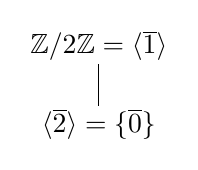
\begin{tikzpicture}[baseline=(current bounding box.center), every node/.style={inner sep=1pt}]
					\node (a) at (0,0.8) {$\ZZ/2\ZZ=\langle \overline{1}\rangle$};
					\node (b) at (0,-0.2) {$\langle\overline{2}\rangle=\{\overline{0}\}$};
					\draw (a)--(b);
				\end{tikzpicture}
			\end{minipage}
			\begin{minipage}{0.42\linewidth}
				\centering
				\begin{tikzpicture}[baseline=(current bounding box.center), every node/.style={inner sep=1pt}]
					\node (a) at (0,1.2) {$\ZZ/4\ZZ=\langle \overline{1}\rangle$};
					\node (note) at (2.5,1.2) {\small（注意：$\langle\overline{1}\rangle=\langle\overline{3}\rangle$）};
					\node (b) at (0,0.1) {$\langle\overline{2}\rangle$};
					\node (c) at (0,-1.0) {$\langle\overline{4}\rangle=\{\overline{0}\}$};
					\draw (a)--(b)--(c);
				\end{tikzpicture}
			\end{minipage}
		\end{center}
		
		\begin{center}
			\begin{tikzpicture}[every node/.style={inner sep=1pt}]
				\node (a) at (0,1.8) {$\ZZ/8\ZZ=\langle\overline{1}\rangle$};
				\node (note) at (3.8,1.8) {\small（注意：$\langle\overline{1}\rangle=\langle\overline{3}\rangle=\langle\overline{5}\rangle=\langle\overline{7}\rangle$）};
				\node (b) at (0,0.7) {$\langle\overline{2}\rangle$};
				\node (c) at (0,-0.4) {$\langle\overline{4}\rangle$};
				\node (d) at (0,-1.5) {$\langle\overline{8}\rangle=\{\overline{0}\}$};
				\draw (a)--(b)--(c)--(d);
			\end{tikzpicture}
		\end{center}
		
		一般地，若 $p$ 是素数，则 $\ZZ/p^n\ZZ$ 的格为
		\begin{center}
			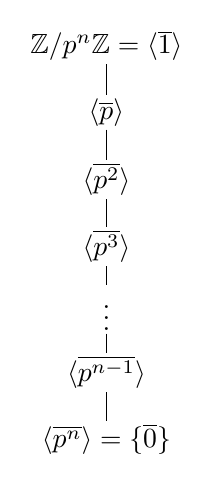
\begin{tikzpicture}[every node/.style={inner sep=1pt}]
				\node (a) at (0,2.8) {$\ZZ/p^n\ZZ=\langle\overline{1}\rangle$};
				\node (b) at (0,1.95) {$\langle\overline{p}\rangle$};
				\node (c) at (0,1.1) {$\langle\overline{p^2}\rangle$};
				\node (d) at (0,0.25) {$\langle\overline{p^3}\rangle$};
				\node (e) at (0,-0.55) {$\vdots$};
				\node (f) at (0,-1.35) {$\langle\overline{p^{n-1}}\rangle$};
				\node (g) at (0,-2.2) {$\langle\overline{p^n}\rangle=\{\overline{0}\}$};
				\draw (a)--(b)--(c)--(d)--(e)--(f)--(g);
			\end{tikzpicture}
		\end{center}
		
		\begin{center}
			\begin{minipage}{0.45\linewidth}
				\centering
				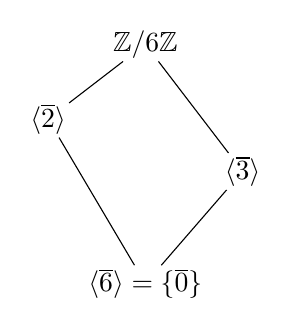
\begin{tikzpicture}[scale=.95, every node/.style={inner sep=1pt}]
					\node (top) at (0,2) {$\ZZ/6\ZZ$};
					\node (a) at (-1.3,1) {$\langle\overline{2}\rangle$};
					\node (b) at (1.3,0.3) {$\langle\overline{3}\rangle$};
					\node (bot) at (0,-1.2) {$\langle\overline{6}\rangle=\{\overline{0}\}$};
					\draw (top)--(a)--(bot)--(b)--(top);
				\end{tikzpicture}
			\end{minipage}
			\begin{minipage}{0.45\linewidth}
				\centering
				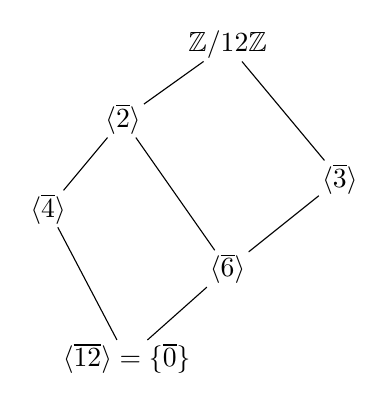
\begin{tikzpicture}[scale=.95, every node/.style={inner sep=1pt}]
					\node (top) at (0,2.2) {$\ZZ/12\ZZ$};
					\node (a) at (-1.4,1.2) {$\langle\overline{2}\rangle$};
					\node (b) at (1.5,.4) {$\langle\overline{3}\rangle$};
					\node (c) at (-2.4,0) {$\langle\overline{4}\rangle$};
					\node (d) at (0,-.8) {$\langle\overline{6}\rangle$};
					\node (bot) at (-1.35,-2.0) {$\langle\overline{12}\rangle=\{\overline{0}\}$};
					\draw (top)--(a)--(c)--(bot)--(d)--(b)--(top);
					\draw (a)--(d);
				\end{tikzpicture}
			\end{minipage}
		\end{center}
		\item \textbf{克莱因四元群}（Viergruppe）$V_4$ 是阶为 $4$ 的群，其乘法表与格为
		\begin{center}
			\begin{tabular}{c@{\qquad}c}
				$\begin{array}{c|cccc}
					\cdot&1&a&b&c\\ \hline
					1&1&a&b&c\\
					a&a&1&c&b\\
					b&b&c&1&a\\
					c&c&b&a&1
				\end{array}$
				&
				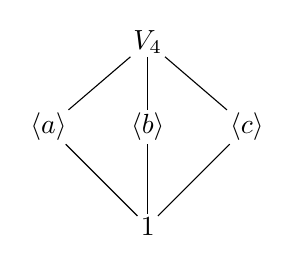
\begin{tikzpicture}[baseline=(current bounding box.center), scale=.9, every node/.style={inner sep=1pt}]
					\node (top) at (0,2) {$V_4$};
					\node (a) at (-1.4,.8) {$\langle a\rangle$};
					\node (b) at (0,.8) {$\langle b\rangle$};
					\node (c) at (1.4,.8) {$\langle c\rangle$};
					\node (bot) at (0,-.6) {$1$};
					\draw (top)--(a)--(bot)--(c)--(top);
					\draw (top)--(b)--(bot);
				\end{tikzpicture}
			\end{tabular}
		\end{center}
		注意 $V_4$ 是阿贝尔群，且不同构于 $Z_4$。我们会看到 $D_8$ 含有一个同构于 $V_4$ 的子群，因此不必检查上述定义的二元运算满足结合律。
		
		\item $S_3$ 的格为
		\begin{center}
			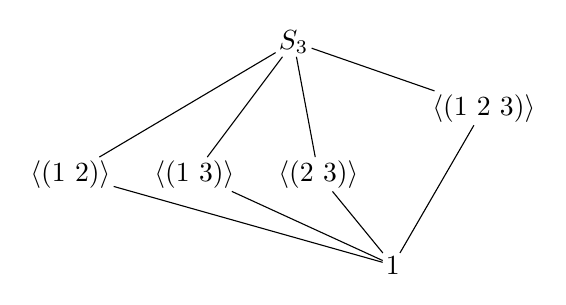
\begin{tikzpicture}[scale=1.05, every node/.style={inner sep=1pt}]
				\node (top) at (0,2.2) {$S_3$};
				\node (a) at (-2.7,.6) {$\langle(1\ 2)\rangle$};
				\node (b) at (-1.2,.6) {$\langle(1\ 3)\rangle$};
				\node (c) at (.3,.6) {$\langle(2\ 3)\rangle$};
				\node (d) at (2.3,1.4) {$\langle(1\ 2\ 3)\rangle$};
				\node (bot) at (1.2,-.5) {$1$};
				\foreach \x in {a,b,c,d} {\draw (top)--(\x); \draw (\x)--(bot);}
			\end{tikzpicture}
		\end{center}
		
		\item 用通常记号 $D_8=\langle r,s\rangle$，$D_8$ 的格为
		\begin{center}
		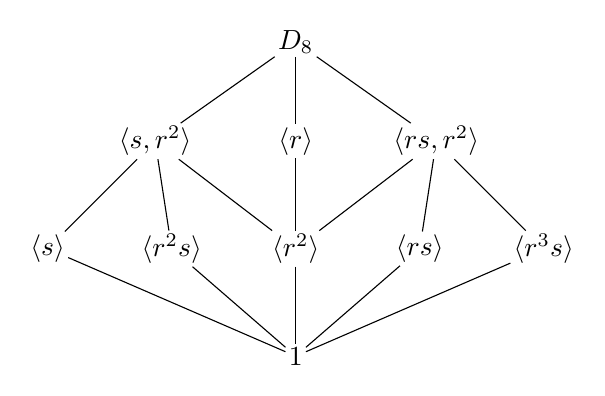
\begin{tikzpicture}[scale=1.05, every node/.style={inner sep=1pt}]
			\node (top) at (0,3) {$D_8$};
			\node (a) at (-1.7,1.8) {$\langle s,r^2\rangle$};
			\node (b) at (0,1.8) {$\langle r\rangle$};
			\node (c) at (1.7,1.8) {$\langle rs,r^2\rangle$};
			\node (d) at (-3,.5) {$\langle s\rangle$};
			\node (e) at (-1.5,.5) {$\langle r^2s\rangle$};
			\node (f) at (0,.5) {$\langle r^2\rangle$};
			\node (g) at (1.5,.5) {$\langle rs\rangle$};
			\node (h) at (3,.5) {$\langle r^3s\rangle$};
			\node (bot) at (0,-.8) {$1$};
			\draw (top)--(a)--(d)--(bot);
			\draw (top)--(b)--(f)--(bot);
			\draw (top)--(c)--(h)--(bot);
			\draw (a)--(e)--(bot);
			\draw (a)--(f);
			\draw (c)--(f);
			\draw (c)--(g)--(bot);
		\end{tikzpicture}
		\end{center}
		\item $D_{16}$ 的子群格不是平面图（不能在平面上画出而不使线相交）。它的一种画法是
		\begin{center}
			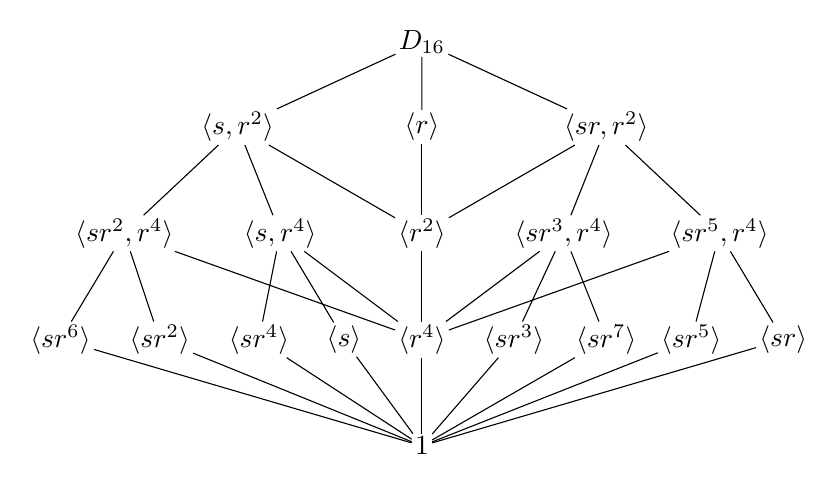
\begin{tikzpicture}[scale=.9, every node/.style={inner sep=1pt}]
				\node (top) at (0,5) {$D_{16}$};
				\node (sr2) at (-2.6,3.8) {$\langle s,r^2\rangle$};
				\node (r) at (0,3.8) {$\langle r\rangle$};
				\node (srr2) at (2.6,3.8) {$\langle sr,r^2\rangle$};
				\node (sr2r4) at (-4.2,2.3) {$\langle sr^2,r^4\rangle$};
				\node (sr4) at (-2,2.3) {$\langle s,r^4\rangle$};
				\node (r2) at (0,2.3) {$\langle r^2\rangle$};
				\node (sr3r4) at (2,2.3) {$\langle sr^3,r^4\rangle$};
				\node (sr5r4) at (4.2,2.3) {$\langle sr^5,r^4\rangle$};
				\node (sr6) at (-5.1,.8) {$\langle sr^6\rangle$};
				\node (sr2s) at (-3.7,.8) {$\langle sr^2\rangle$};
				\node (sr4s) at (-2.3,.8) {$\langle sr^4\rangle$};
				\node (ss) at (-1.1,.8) {$\langle s\rangle$};
				\node (r4) at (0,.8) {$\langle r^4\rangle$};
				\node (sr3) at (1.3,.8) {$\langle sr^3\rangle$};
				\node (sr7) at (2.6,.8) {$\langle sr^7\rangle$};
				\node (sr5) at (3.8,.8) {$\langle sr^5\rangle$};
				\node (sr) at (5.1,.8) {$\langle sr\rangle$};
				\node (bot) at (0,-.7) {$1$};
				\draw (top)--(sr2) (top)--(r) (top)--(srr2);
				\draw (sr2)--(sr2r4) (sr2)--(sr4) (sr2)--(r2);
				\draw (r)--(r2);
				\draw (srr2)--(r2) (srr2)--(sr3r4) (srr2)--(sr5r4);
				\draw (sr2r4)--(sr6) (sr2r4)--(sr2s) (sr2r4)--(r4);
				\draw (sr4)--(sr4s) (sr4)--(ss) (sr4)--(r4);
				\draw (r2)--(r4);
				\draw (sr3r4)--(r4) (sr3r4)--(sr3) (sr3r4)--(sr7);
				\draw (sr5r4)--(r4) (sr5r4)--(sr5) (sr5r4)--(sr);
				\foreach \x in {sr6,sr2s,sr4s,ss,r4,sr3,sr7,sr5,sr} {\draw (\x)--(bot);}
			\end{tikzpicture}
		\end{center}
	\end{enumerate}
	
	
\end{example}


在理论证明和具体例子中，我们常常只关心给定群的两个（或少数几个）子群及其相互关系。为了把这些关系画出来，我们将画出整个群格的一个\textbf{子格}，其中包含相关的上确界与交。这样的子格中的一条不断开的线一般并不表示该线两端之间没有其他子群。这些部分格也会在处理无限群时使用。例如，若只想讨论 $D_{16}$ 的子群 $\langle sr^2,r^4\rangle$ 与 $\langle r^2\rangle$ 的关系，可画出如下子格：
\begin{center}
	\begin{tikzpicture}[scale=1.0, every node/.style={inner sep=1pt}]
		\node (top) at (0,4) {$D_{16}$};
		\node (a) at (0,3) {$\langle s,r^2\rangle$};
		\node (b) at (-1.5,1.8) {$\langle sr^2,r^4\rangle$};
		\node (c) at (1.5,1.8) {$\langle r^2\rangle$};
		\node (d) at (0,.6) {$\langle r^4\rangle$};
		\node (bot) at (0,-.5) {$1$};
		\draw (top)--(a)--(b)--(d)--(bot);
		\draw (a)--(c)--(d);
	\end{tikzpicture}
\end{center}
注意 $\langle s,r^2\rangle$ 和 $\langle r^4\rangle$ 分别正是这两个子群在 $D_{16}$ 中的上确界与交。

最后，给定一个群的子群格后，计算正规化子和中心化子相对容易。例如，在 $D_8$ 中，可以看出 $C_{D_8}(s)=\langle s,r^2\rangle$，因为先计算得 $r^2\in C_{D_8}(s)$（见第 2 节）。这证明 $\langle s,r^2\rangle\leq C_{D_8}(s)$（注意一个元素总属于它自身的中心化子）。包含 $\langle s,r^2\rangle$ 的子群只有它自身和整个 $D_8$。不可能有 $C_{D_8}(s)=D_8$，因为 $r$ 不与 $s$ 交换（即 $r\notin C_{D_8}(s)$）。于是只剩所声称的一种可能。



% !TEX root = ../main.tex
\setchapterimage{}
\setchapterintro{}
\chapter{商群与同态}

\section{商群}
本章引入群 $G$ 的\textbf{商群}概念，这是从群 $G$ 得到一个“较小”群的另一种方法；正如我们对待子群那样，我们将用商群来研究 $G$ 的结构。
\begin{definition}
	若 $\varphi$ 是从 $G$ 到群 $H$ 的同态，则 $\varphi$ 的\textbf{纤维}是 $G$ 中映到 $H$ 的单个元素上的元素集合。
	
	就是说$\varphi$ 在 $a\in H$ 上方的纤维定义为
	\[\{x\in G :\varphi (x) = a\in H\}\]
\end{definition}
	可以把这种情形图示为图 1，其中点 $a$ 上方方框中的竖线表示 $\varphi$ 在 $a$ 上方的纤维。
\begin{center}
	\begin{tikzpicture}[scale=.95, every node/.style={inner sep=1pt}]
		\draw (-3.8,1) rectangle (3.8,2.4);
		\foreach \x in {-3.1,-2.8,-.55,.55,2.8,3.1}{\draw (\x,1.15)--(\x,2.25);} 
		\node at (-1.65,1.7) {$\cdots$};
		\node at (1.65,1.7) {$\cdots$};
		\node[right] at (4.0,1.7) {$G$};
		\draw (-3.8,0)--(3.8,0);
		\foreach \x in {-3.1,-2.8,0,2.8,3.1}{\fill (\x,0) circle (1.7pt);}
		\foreach \x in {-3.1,-2.8,0,2.8,3.1}{\draw[->] (\x,1.0)--(\x,.13);} 
		\node[below] at (0,0) {$a$};
		\node[right] at (4.0,0) {$H$};
		\node at (3.95,-.55) {图 1};
	\end{tikzpicture}
\end{center}

$H$ 中的群运算给出一种方法来相乘 $\varphi$ 的像中的两个元素。若 $X_a$ 是 $a$ 上方的纤维，$X_b$ 是 $b$ 上方的纤维，则定义 $X_a$ 与 $X_b$ 的乘积为 $ab$ 上方的纤维 $X_{ab}$，即
\[
X_aX_b=X_{ab}.
\]
这种乘法是结合的，因为 $H$ 中的乘法结合；单位元是 $H$ 的单位元上方的纤维；$a$ 上方纤维的逆是 $a^{-1}$ 上方的纤维。例如，结合律证明如下：
\[
(X_aX_b)X_c=(X_{ab})X_c=X_{(ab)c},\qquad
X_a(X_bX_c)=X_a(X_{bc})=X_{a(bc)}.
\]
由于 $(ab)c=a(bc)$ 在 $H$ 中成立，故 $(X_aX_b)X_c=X_a(X_bX_c)$。粗略地说，群 $G$ 被分划成若干片（纤维），而这些片本身具有群结构，称为 $G$ 的商群（正式定义见下面）。

\begin{definition}
	 若 $\varphi:G\to H$ 是同态，则 $\varphi$ 的\textbf{核}是集合
	\[
	\{g\in G\mid \varphi(g)=1\},
	\]
	记为 $\ker\varphi$（这里 $1$ 是 $H$ 的单位元）。
\end{definition}
\begin{proposition}\label{核的群性质}
	设 $G$ 和 $H$ 是群，$\varphi:G\to H$ 是同态。
	\begin{enumerate}[label=(\arabic*)]
		\item $\varphi(1_G)=1_H$，其中 $1_G$ 与 $1_H$ 分别为 $G$ 与 $H$ 的单位元。
		\item 对所有 $g\in G$，$\varphi(g^{-1})=\varphi(g)^{-1}$。
		\item 对所有 $n\in\ZZ$，$\varphi(g^n)=\varphi(g)^n$。
		\item $\ker\varphi$ 是 $G$ 的子群。
		\item $\im(\varphi)$，即 $G$ 在 $\varphi$ 下的像，是 $H$ 的子群。
	\end{enumerate}
\end{proposition}
\begin{proof}
	(1) 由于
	\[
	\varphi(1_G)=\varphi(1_G1_G)=\varphi(1_G)\varphi(1_G),
	\]
	由消去律得 $\varphi(1_G)=1_H$。
	
	(2) 由 (1)，
	\[
	1_H=\varphi(1_G)=\varphi(gg^{-1})=\varphi(g)\varphi(g^{-1}).
	\]
	左乘 $\varphi(g)^{-1}$ 并化简，得结论。
	
	(3) 当 $n\in\ZZ^+$ 时由归纳法即可；负整数情形由 (2) 推出。
	
	(4) 由 (1)，$1_G\in\ker\varphi$，所以核非空。若 $x,y\in\ker\varphi$，则 $\varphi(x)=\varphi(y)=1_H$，于是
	\[
	\varphi(xy^{-1})=\varphi(x)\varphi(y^{-1})
	=\varphi(x)\varphi(y)^{-1}=1_H1_H^{-1}=1_H.
	\]
	所以 $xy^{-1}\in\ker\varphi$。由子群判别法，$\ker\varphi\leq G$。
	
	(5) 由 $\varphi(1_G)=1_H$，$H$ 的单位元属于 $\im(\varphi)$。若 $x,y\in\im(\varphi)$，设 $x=\varphi(a)$，$y=\varphi(b)$，则由 (2)，$y^{-1}=\varphi(b^{-1})$，所以
	\[
	xy^{-1}=\varphi(a)\varphi(b^{-1})=\varphi(ab^{-1})
	\]
	仍在像中。由子群判别法，$\im(\varphi)\leq H$。
\end{proof}

\begin{definition}
	设 $\varphi:G\to H$ 是同态，其核为 $K$。\textbf{商群}或\textbf{因子群} $G/K$（读作 $G$ 模 $K$，或简称 $G$ mod $K$）是一个群，其元素是 $\varphi$ 的纤维，群运算定义如上：若 $X$ 是 $a$ 上方的纤维，$Y$ 是 $b$ 上方的纤维，则 $X$ 与 $Y$ 的乘积定义为 $ab$ 上方的纤维。
\end{definition}

\begin{proposition}\label{核的左右陪集相等}
	设 $\varphi:G\to H$ 是群同态，核为 $K$。设 $X\in G/K$ 是 $a$ 上方的纤维，即 $X=\varphi^{-1}(a)$。则
\begin{enumerate}[label=(\arabic*)]
	\item 对任意 $u\in X$，有 $X=\{uk\mid k\in K\}$；
	\item 对任意 $u\in X$，有 $X=\{ku\mid k\in K\}$。
\end{enumerate}
\end{proposition}
\begin{proof}
	(1) 取 $u\in X$，于是 $\varphi(u)=a$。令
	\[
	uK=\{uk\mid k\in K\}.
	\]
	先证 $uK\subseteq X$。若 $k\in K$，则
	\[
	\varphi(uk)=\varphi(u)\varphi(k)=\varphi(u)1=a,
	\]
	所以 $uk\in X$。反过来，设 $g\in X$，令 $k=u^{-1}g$。则
	\[
	\varphi(k)=\varphi(u^{-1})\varphi(g)=\varphi(u)^{-1}\varphi(g)=a^{-1}a=1.
	\]
	因此 $k\in K$。又 $k=u^{-1}g$，故 $g=uk\in uK$。于是 $X=uK$。
	
	(2) 类似地，取 $u\in X$， $\varphi(u)=a$。令
	\[
	Ku=\{ku\mid k\in K\}.
	\]
	先证 $Ku\subseteq X$。若 $k\in K$，则
	\[
	\varphi(ku)=\varphi(k)\varphi(u)=1\varphi(u)=a,
	\]
	所以 $ku\in X$。反过来，设 $g\in X$，令 $k=gu^{-1}$。则
	\[
	\varphi(k)=\varphi(g)\varphi(u^{-1})=\varphi(g)\varphi(u)^{-1}=aa^{-1}=1.
	\]
	因此 $k\in K$。又 $k=gu^{-1}$，故 $g=ku\in Ku$。于是 $X=Ku$。
\end{proof}
综上，我们看到了对一个同态$\varphi $的核$K$，其在$a$上的纤维有
\[X = uK = Ku,\qquad u\in X\]

\begin{definition}
	任意 $N\leq G$ 和任意 $g\in G$，令
\[
gN=\{gn\mid n\in N\},\qquad Ng=\{ng\mid n\in N\},
\]
分别称为 $N$ 在 $G$ 中的\textbf{左陪集}和\textbf{右陪集}。陪集中的任意元素称为该陪集的一个\textbf{代表元}。

\end{definition}
若 $G$ 是加法群，我们写 $g+N$ 和 $N+g$ 分别表示代表元为 $g$ 的左、右陪集。一般地，可把左陪集 $gN$ 看作 $N$ 被 $g$ 左平移所得的集合。


用这个定义来说，\ref{核的左右陪集相等}表明同态的纤维是核的左陪集（也是核的右陪集），即商 $G/K$ 的元素是左陪集 $gK$，$g\in G$。



\begin{proposition}\label{陪集的乘积是良定的}
	设 $G$ 是群，$K$ 是从 $G$ 到另一群的某个同态的核。则 $K$ 在 $G$ 中的左陪集组成的集合，在运算
\[
uK\circ vK=(uv)K
\]
下构成群 $G/K$。特别地，此运算是良定义的：若 $u_1$ 是 $uK$ 中任意元素，$v_1$ 是 $vK$ 中任意元素，则 $u_1v_1\in uvK$，即 $u_1v_1K=uvK$，所以乘法不依赖于陪集代表元的选择。把“左陪集”换成“右陪集”也有相同结论
\end{proposition}

\begin{proof}
	设 $X,Y\in G/K$，令 $Z=XY$。由\ref{核的左右陪集相等}(1)，$X,Y,Z$ 都是 $K$ 的左陪集。按假设，$K$ 是某个同态 $\varphi:G\to H$ 的核，所以 $X=\varphi^{-1}(a)$，$Y=\varphi^{-1}(b)$，其中 $a,b\in H$。根据 $G/K$ 中的运算定义，$Z=\varphi^{-1}(ab)$。任取 $X$、$Y$ 的代表元 $u$、$v$，则 $\varphi(u)=a$，$\varphi(v)=b$，且 $X=uK$、$Y=vK$。要证 $uv\in Z$。确实，
	\[
	uv\in Z \Longleftrightarrow uv\in\varphi^{-1}(ab)
	\Longleftrightarrow \varphi(uv)=ab
	\Longleftrightarrow \varphi(u)\varphi(v)=ab,
	\]
	而最后一个等式成立。故 $uv\in Z$，因此 $Z=uvK$。这证明了对任意代表元 $u\in X$、$v\in Y$，$X$ 与 $Y$ 的乘积都是陪集 $uvK$。最后关于右陪集的断言由\ref{核的左右陪集相等} 中 $uK=Ku$、$vK=Kv$ 立即推出。
\end{proof}

用代表元作 $G/K$ 中的乘法，可如图 3 所示。

\begin{center}
	\begin{tikzpicture}[scale=.9, every node/.style={inner sep=1pt}]
		\draw (-3.8,1) rectangle (3.8,2.55);
		\foreach \x in {-3.1,-.6,2.6}{\draw (\x,1.1)--(\x,2.45);} 
		\node at (.85,1.78) {$\cdots$};
		\node at (-3.1,2.62) {$u$}; \node at (-.6,2.62) {$v$}; \node at (2.6,2.62) {$uv$};
		\draw[dashed,->] (-3.0,2.35) .. controls (-2.0,2.95) and (-1.2,2.95) .. (-.65,2.35);
		\draw[dashed,->] (-.55,2.35) .. controls (.4,2.95) and (1.7,2.95) .. (2.55,2.35);
		\node[right] at (4.0,1.78) {$G$};
		\draw (-3.8,0)--(3.8,0);
		\foreach \x/\lab in {-3.1/a,-.6/b,2.6/ab}{\fill (\x,0) circle (1.7pt); \node[below] at (\x,0) {$\lab$}; \draw[->] (\x,1.0)--(\x,.13);} 
		\draw[dashed,->] (-3.0,.3) .. controls (-2.0,.75) and (1.2,.75) .. (2.55,.3);
		\draw[dashed,->] (-.55,.25) .. controls (.6,.55) and (1.55,.55) .. (2.55,.25);
		\node[right] at (4.0,0) {$H$};
		\node at (3.9,-.55) {图 3};
	\end{tikzpicture}
\end{center}

由定理\ref{陪集的乘积是良定的}，若给定群 $G$ 的子群 $K$，并知道 $K$ 是某个同态的核，则可不借助该同态而通过乘法 $uK\cdot vK=uvK$ 定义商 $G/K$。这引出一个问题：是否可对 $G$ 的任意子群 $N$ 都类似地定义商群 $G/N$？答案一般是否定的，因为这种乘法一般不是良定义的。
\begin{proposition}\label{一般子群的陪集}
	设 $N$ 是群 $G$ 的任意子群。$N$ 在 $G$ 中的左陪集组成 $G$ 的一个\textbf{分划}\footnote{也就是说，$G$可以被分成$N$ 在 $G$ 中的左陪集的不交并.}。此外，对所有 $u,v\in G$，
	\[
	uN=vN\quad\Longleftrightarrow\quad v^{-1}u\in N,
	\]
	特别地，$uN=vN$ 当且仅当 $u$ 和 $v$ 是同一陪集的代表元。
\end{proposition}
\begin{proof}
	首先，由于 $N$ 是 $G$ 的子群，$1\in N$。因此对所有 $g\in G$，$g=g\cdot1\in gN$，所以
	\[
	G=\bigcup_{g\in G} gN.
	\]
	为证明不同左陪集不交，设 $uN\cap vN\neq\varnothing$。取 $x\in uN\cap vN$，写作
	\[
	x=un=vm,
	\]
	其中 $n,m\in N$。在等式右端两边右乘 $n^{-1}$，得
	\[
	u=vmn^{-1}=vm_1,
	\]
	其中 $m_1=mn^{-1}\in N$。于是对 $uN$ 的任意元素 $ut$（$t\in N$），有
	\[
	ut=(vm_1)t=v(m_1t)\in vN.
	\]
	故 $uN\subseteq vN$。交换 $u$ 与 $v$ 可得 $vN\subseteq uN$。因此有非空交的两个陪集相等。
	
	由前面的结论，$uN=vN$ 当且仅当 $u\in vN$，当且仅当 $u=vn$ 对某个 $n\in N$ 成立，当且仅当 $v^{-1}u\in N$。最后，$v\in uN$ 等价于说 $v$ 是 $uN$ 的代表元，所以 $uN=vN$ 当且仅当 $u$ 与 $v$ 是同一个陪集的代表元。
\end{proof}

\begin{proposition}\label{一般子群的陪集成群的充要条件}
	设 $G$ 是群，$N$ 是 $G$ 的子群。
	\begin{enumerate}[label=(\arabic*)]
		\item 在 $N$ 的左陪集集合上由
		\[
		uN\cdot vN=(uv)N
		\]
		描述的运算是良定义的，当且仅当对所有 $g\in G$ 和所有 $n\in N$，都有 $gng^{-1}\in N$。
		\item 若上述运算是良定义的，则它使 $N$ 的左陪集集合成为一个群。特别地，该群的单位元是陪集 $1N$，$gN$ 的逆是 $g^{-1}N$，即 $(gN)^{-1}=g^{-1}N$。
	\end{enumerate}
\end{proposition}

\begin{proof}
	(1) 先假设该运算良定义。取任意 $g\in G$ 与 $n\in N$。
	\[gng^{-1}\in \iff ng^{-1}N=g^{-1}N\iff N\cdot g^{-1}N=g^{-1}N\]
	令 $u=1$，$u_1=n$，且 $v=v_1=g^{-1}$。由良定义性得
	\[
	1g^{-1}N=ng^{-1}N,
	\]
	即 $g^{-1}N=ng^{-1}N$。由于 $1\in N$，$ng^{-1}\in ng^{-1}N$，所以 $ng^{-1}\in g^{-1}N$，即 $ng^{-1}=g^{-1}n_1$，其中 $n_1\in N$。左乘 $g$，得 $gng^{-1}=n_1\in N$。
	
	反过来，假设 $gng^{-1}\in N$ 对所有 $g\in G$ 和 $n\in N$ 成立。设 $u_1\in uN$，$v_1\in vN$。写作 $u_1=un$，$v_1=vm$，其中 $n,m\in N$。要证 $u_1v_1\in uvN$：
	\[
	u_1v_1=(un)(vm)=u(vv^{-1})nvm=(uv)(v^{-1}nv)m=(uv)(n_1m),
	\]
	其中 $n_1=v^{-1}nv\in N$。由于 $N$ 对乘积封闭，$n_1m\in N$。故 $u_1v_1=(uv)n_2$，其中 $n_2\in N$。于是左陪集 $uvN$ 与 $u_1v_1N$ 有公共元素 $u_1v_1$，由\ref{一般子群的陪集} 它们相等。运算良定义。
	
	(2) 若陪集上的运算良定义，则群公理由 $G$ 中对应公理诱导。例如，对所有 $u,v,w\in G$，
	\begin{align*}
		(uN)(vNwN)&=uN(vwN)=u(vw)N\\
		&=(uv)wN=(uNvN)(wN),
	\end{align*}
	因为 $u(vw)=(uv)w$ 在 $G$ 中成立。由乘法定义可立即看出单位元是 $1N$，$gN$ 的逆是 $g^{-1}N$。
\end{proof}



\begin{definition}
	 元素 $gng^{-1}$ 称为 $n\in N$ 关于 $g$ 的\textbf{共轭}。集合
\[
gNg^{-1}=\{gng^{-1}\mid n\in N\}
\]
称为 $N$ 关于 $g$ 的\textbf{共轭}。若 $gNg^{-1}=N$，则称 $g$ \textbf{正规化} $N$。群 $G$ 的子群 $N$ 称为\textbf{正规子群}，如果 $G$ 的每个元素都正规化 $N$，即对所有 $g\in G$ 都有 $gNg^{-1}=N$。若 $N$ 是 $G$ 的正规子群，记为 $N\normal G$。

\end{definition}
\textbf{注意，}当 $N$ 是正规子群时，$G$ 的结构反映在商 $G/N$ 的结构中（例如，$G/N$ 中乘法的结合律由 $G$ 中的结合律诱导，$G/N$ 中的逆由 $G$ 中的逆诱导）。第 3 节讨论同构定理时，我们会看到更多 $G$ 与其商 $G/N$ 的关系。

\begin{theorem}
	设 $N$ 是群 $G$ 的子群。以下条件等价：
\begin{enumerate}[label=(\arabic*)]
	\item $N\normal G$；
	\item $N_G(N)=G$；
	\item 对所有 $g\in G$，$gN=Ng$；
	\item 命题 5 中描述的左陪集运算使左陪集集合成为群；
	\item 对所有 $g\in G$，$gNg^{-1}\subseteq N$。
\end{enumerate}

\end{theorem}



















%% !TEX root = ../main.tex
\setchapterimage{}
\setchapterintro{}
\chapter{群作用}

\section{群作用的定义}
% TODO

%% !TEX root = ../main.tex
\setchapterimage{}
\setchapterintro{}
\chapter{直积、半直积与 Abel 群}

\section{直积与直和}
% TODO

%% !TEX root = ../main.tex
\setchapterimage{}
\setchapterintro{}
\chapter{群论进阶专题}

\section{Sylow 定理}
% TODO

%
%% ═══════════════════════════════════════════════════════
%%  Part II：环论 (Ring Theory)
%% ═══════════════════════════════════════════════════════
%\setpartimage{}
%\setpartintro{从环的公理化定义切入，研究整环、理想、商环、同态基本定理，并深入 Euclid 整环、主理想整环与唯一分解整环的结构理论。}
%\part{环论}
%
%% !TEX root = ../main.tex
\setchapterimage{}
\setchapterintro{}
\chapter{环论导引}

\section{环的定义与例子}
% TODO

%% !TEX root = ../main.tex
\setchapterimage{}
\setchapterintro{}
\chapter{Euclid 整环、主理想整环与唯一分解整环}

\section{Euclid 整环}
% TODO

%% !TEX root = ../main.tex
\setchapterimage{}
\setchapterintro{}
\chapter{多项式环}

\section{单变量多项式环}
% TODO

%
%% ═══════════════════════════════════════════════════════
%%  Part III：模与向量空间 (Modules and Vector Spaces)
%% ═══════════════════════════════════════════════════════
%\setpartimage{}
%\setpartintro{模是环上「线性代数」的自然推广。从模的基本概念出发，研究自由模、向量空间的深入性质，以及主理想整环上有限生成模的结构定理。}
%\part{模与向量空间}
%
%% !TEX root = ../main.tex
\setchapterimage{}
\setchapterintro{}
\chapter{模论导引}

\section{模的定义与例子}
% TODO

%% !TEX root = ../main.tex
\setchapterimage{}
\setchapterintro{}
\chapter{向量空间}

\section{向量空间的定义与基}
% TODO

%% !TEX root = ../main.tex
\setchapterimage{}
\setchapterintro{}
\chapter{主理想整环上的模}

\section{主理想整环上有限生成模的结构定理}
% TODO

%
%% ═══════════════════════════════════════════════════════
%%  Part IV：域论与 Galois 理论 (Field Theory and Galois Theory)
%% ═══════════════════════════════════════════════════════
%\setpartimage{}
%\setpartintro{域扩张与 Galois 理论是抽象代数的华彩乐章。从域的代数扩张到 Galois 群与 Galois 对应，最终解决古典的方程根式可解性问题。}
%\part{域论与 Galois 理论}
%
%% !TEX root = ../main.tex
\setchapterimage{}
\setchapterintro{}
\chapter{域论}

\section{域扩张}
% TODO

%% !TEX root = ../main.tex
\setchapterimage{}
\setchapterintro{}
\chapter{Galois 理论}

\section{Galois 扩张与 Galois 群}
% TODO

%
%% ═══════════════════════════════════════════════════════
%%  Part V：交换环、代数几何与同调代数导引
%% ═══════════════════════════════════════════════════════
%\setpartimage{}
%\setpartintro{从交换环的局部化与整闭包出发，探索 Noether 环、仿射代数集与 Hilbert 零点定理，并学习 Artin 环、投射模、内射模及同调代数的初步工具。}
%\part{交换环、代数几何与同调代数导引}
%
%% !TEX root = ../main.tex
\setchapterimage{}
\setchapterintro{}
\chapter{交换环与代数几何}

\section{Noether 环与 Hilbert 基定理}
% TODO

%% !TEX root = ../main.tex
\setchapterimage{}
\setchapterintro{}
\chapter{Artin 环、投射模与内射模}

\section{Artin 环}
% TODO

%% !TEX root = ../main.tex
\setchapterimage{}
\setchapterintro{}
\chapter{同调代数与群上同调导引}

\section{链复形与同调}
% TODO

%
%% ═══════════════════════════════════════════════════════
%%  Part VI：有限群表示论导引
%% ═══════════════════════════════════════════════════════
%\setpartimage{}
%\setpartintro{用线性代数的方法研究有限群的结构。从群表示与特征标的基本理论出发，通过大量实例展现表示论在群论中的强大应用。}
%\part{有限群表示论导引}
%
%% !TEX root = ../main.tex
\setchapterimage{}
\setchapterintro{}
\chapter{表示论与特征标理论}

\section{群表示的定义}
% TODO

%% !TEX root = ../main.tex
\setchapterimage{}
\setchapterintro{}
\chapter{特征标理论的例子与应用}

\section{特征标表的计算}
% TODO



\backmatter
\nocite{dummit_abstract_2004}
\bibliographystyle{IEEEtran}
\bibliography{bibliography/references}

\end{document}
